%!TEX TS-program = xelatex
\documentclass[10pt,oneside]{article}
\usepackage[fontsize=9pt]{scrextend}

\usepackage[english]{babel}

\usepackage{amsmath,amssymb,amsfonts}
\usepackage[utf8]{inputenc}
\usepackage[T1]{fontenc}
\usepackage{stix2}
\usepackage[scaled]{helvet}
\usepackage[scaled]{inconsolata}

\usepackage{lastpage}

\usepackage{setspace}

\usepackage{ccicons}

\usepackage[hang,flushmargin]{footmisc}

\usepackage{geometry}

\setlength{\parindent}{0pt}
\setlength{\parskip}{6pt plus 2pt minus 1pt}

\usepackage{fancyhdr}
\renewcommand{\headrulewidth}{0pt}\providecommand{\tightlist}{%
  \setlength{\itemsep}{0pt}\setlength{\parskip}{0pt}}

\makeatletter
\newcounter{tableno}
\newenvironment{tablenos:no-prefix-table-caption}{
  \caption@ifcompatibility{}{
    \let\oldthetable\thetable
    \let\oldtheHtable\theHtable
    \renewcommand{\thetable}{tableno:\thetableno}
    \renewcommand{\theHtable}{tableno:\thetableno}
    \stepcounter{tableno}
    \captionsetup{labelformat=empty}
  }
}{
  \caption@ifcompatibility{}{
    \captionsetup{labelformat=default}
    \let\thetable\oldthetable
    \let\theHtable\oldtheHtable
    \addtocounter{table}{-1}
  }
}
\makeatother

\usepackage{array}
\newcommand{\PreserveBackslash}[1]{\let\temp=\\#1\let\\=\temp}
\let\PBS=\PreserveBackslash

\usepackage[breaklinks=true]{hyperref}
\hypersetup{colorlinks,%
citecolor=blue,%
filecolor=blue,%
linkcolor=blue,%
urlcolor=blue}
\usepackage{url}

\usepackage{caption}
\setcounter{secnumdepth}{0}
\usepackage{cleveref}

\usepackage{graphicx}
\makeatletter
\def\maxwidth{\ifdim\Gin@nat@width>\linewidth\linewidth
\else\Gin@nat@width\fi}
\makeatother
\let\Oldincludegraphics\includegraphics
\renewcommand{\includegraphics}[1]{\Oldincludegraphics[width=\maxwidth]{#1}}

\usepackage{longtable}
\usepackage{booktabs}

\usepackage{color}
\usepackage{fancyvrb}
\newcommand{\VerbBar}{|}
\newcommand{\VERB}{\Verb[commandchars=\\\{\}]}
\DefineVerbatimEnvironment{Highlighting}{Verbatim}{commandchars=\\\{\}}
% Add ',fontsize=\small' for more characters per line
\usepackage{framed}
\definecolor{shadecolor}{RGB}{248,248,248}
\newenvironment{Shaded}{\begin{snugshade}}{\end{snugshade}}
\newcommand{\KeywordTok}[1]{\textcolor[rgb]{0.13,0.29,0.53}{\textbf{#1}}}
\newcommand{\DataTypeTok}[1]{\textcolor[rgb]{0.13,0.29,0.53}{#1}}
\newcommand{\DecValTok}[1]{\textcolor[rgb]{0.00,0.00,0.81}{#1}}
\newcommand{\BaseNTok}[1]{\textcolor[rgb]{0.00,0.00,0.81}{#1}}
\newcommand{\FloatTok}[1]{\textcolor[rgb]{0.00,0.00,0.81}{#1}}
\newcommand{\ConstantTok}[1]{\textcolor[rgb]{0.00,0.00,0.00}{#1}}
\newcommand{\CharTok}[1]{\textcolor[rgb]{0.31,0.60,0.02}{#1}}
\newcommand{\SpecialCharTok}[1]{\textcolor[rgb]{0.00,0.00,0.00}{#1}}
\newcommand{\StringTok}[1]{\textcolor[rgb]{0.31,0.60,0.02}{#1}}
\newcommand{\VerbatimStringTok}[1]{\textcolor[rgb]{0.31,0.60,0.02}{#1}}
\newcommand{\SpecialStringTok}[1]{\textcolor[rgb]{0.31,0.60,0.02}{#1}}
\newcommand{\ImportTok}[1]{#1}
\newcommand{\CommentTok}[1]{\textcolor[rgb]{0.56,0.35,0.01}{\textit{#1}}}
\newcommand{\DocumentationTok}[1]{\textcolor[rgb]{0.56,0.35,0.01}{\textbf{\textit{#1}}}}
\newcommand{\AnnotationTok}[1]{\textcolor[rgb]{0.56,0.35,0.01}{\textbf{\textit{#1}}}}
\newcommand{\CommentVarTok}[1]{\textcolor[rgb]{0.56,0.35,0.01}{\textbf{\textit{#1}}}}
\newcommand{\OtherTok}[1]{\textcolor[rgb]{0.56,0.35,0.01}{#1}}
\newcommand{\FunctionTok}[1]{\textcolor[rgb]{0.00,0.00,0.00}{#1}}
\newcommand{\VariableTok}[1]{\textcolor[rgb]{0.00,0.00,0.00}{#1}}
\newcommand{\ControlFlowTok}[1]{\textcolor[rgb]{0.13,0.29,0.53}{\textbf{#1}}}
\newcommand{\OperatorTok}[1]{\textcolor[rgb]{0.81,0.36,0.00}{\textbf{#1}}}
\newcommand{\BuiltInTok}[1]{#1}
\newcommand{\ExtensionTok}[1]{#1}
\newcommand{\PreprocessorTok}[1]{\textcolor[rgb]{0.56,0.35,0.01}{\textit{#1}}}
\newcommand{\AttributeTok}[1]{\textcolor[rgb]{0.77,0.63,0.00}{#1}}
\newcommand{\RegionMarkerTok}[1]{#1}
\newcommand{\InformationTok}[1]{\textcolor[rgb]{0.56,0.35,0.01}{\textbf{\textit{#1}}}}
\newcommand{\WarningTok}[1]{\textcolor[rgb]{0.56,0.35,0.01}{\textbf{\textit{#1}}}}
\newcommand{\AlertTok}[1]{\textcolor[rgb]{0.94,0.16,0.16}{#1}}
\newcommand{\ErrorTok}[1]{\textcolor[rgb]{0.64,0.00,0.00}{\textbf{#1}}}
\newcommand{\NormalTok}[1]{#1}

\newlength{\cslhangindent}
\setlength{\cslhangindent}{1.5em}
\newlength{\csllabelwidth}
\setlength{\csllabelwidth}{3em}
\newenvironment{CSLReferences}[3] % #1 hanging-ident, #2 entry spacing
 {% don't indent paragraphs
  \setlength{\parindent}{0pt}
  % turn on hanging indent if param 1 is 1
  \ifodd #1 \everypar{\setlength{\hangindent}{\cslhangindent}}\ignorespaces\fi
  % set entry spacing
  \ifnum #2 > 0
  \setlength{\parskip}{#2\baselineskip}
  \fi
 }%
 {}
\usepackage{calc} % for \widthof, \maxof
\newcommand{\CSLBlock}[1]{#1\hfill\break}
\newcommand{\CSLLeftMargin}[1]{\parbox[t]{\maxof{\widthof{#1}}{\csllabelwidth}}{#1}}
\newcommand{\CSLRightInline}[1]{\parbox[t]{\linewidth}{#1}}
\newcommand{\CSLIndent}[1]{\hspace{\cslhangindent}#1}\usepackage[table,dvipsnames]{xcolor}

\geometry{includemp,
            letterpaper,
            top=2.4cm,
            bottom=2.4cm,
            left=1.0cm,
            right=1.0cm,
            marginparwidth=5cm,
            marginparsep=1.0cm}

\usepackage[singlelinecheck=off]{caption}

\captionsetup{
  font={small},
  labelfont={bf},
  format=plain,
  labelsep=quad
}

\usepackage{floatrow}

\floatsetup[figure]{margins=hangright,
              facing=no,
              capposition=beside,
              capbesideposition={center,outside},
              floatwidth=\textwidth}

% \floatsetup[table]{margins=hangright,
%              facing=no,
%              capposition=beside,
%              capbesideposition={center,outside},
%              floatwidth=\textwidth}

\pagestyle{plain}

\setcounter{secnumdepth}{5}

\usepackage{titlesec}

\titleformat{\section}[block]
{\normalfont\large\sffamily}
{\thesection}{.5em}{\titlerule\\[.8ex]\bfseries}

\titleformat{\subsection}[runin]
{\normalfont\fontseries{b}\selectfont\filright\sffamily}
{\thesubsection.}{.5em}{}

\titleformat{\subsubsection}[runin]
{\normalfont\itshape\rmfamily\bfseries}{\thesubsubsection}{1em}{}

\fancypagestyle{firstpage}
{
   \fancyhf{}
   \renewcommand{\headrulewidth}{0pt}
   \fancyfoot[R]{\footnotesize\ccby}
   \fancyfoot[L]{\footnotesize\sffamily\today}
}

\fancypagestyle{normal}
{
  \fancyhf{}
  \fancyfoot[R]{\footnotesize\sffamily\thepage\ of \pageref*{LastPage}}
}

\usepackage{tikz}
\begin{document}
\tikz [remember picture, overlay] %
\node [shift={(-0.6in,1.1cm)},scale=0.2,opacity=0.4] at (current page.south east)[anchor=south east]{
\includegraphics{logo}};%
\pagestyle{normal}
\thispagestyle{firstpage}

\newcommand{\colorRule}[3][black]{\textcolor[HTML]{#1}{\rule{#2}{#3}}}

\noindent {\LARGE \textbf{\textsf{The coevolutionary mosaic of
betacoronavirus emergence risk}}}

\medskip
\begin{flushleft}
{\small
%
Norma\,Forero Rocio Munoz%
%
\,\textsuperscript{1,2,‡}, %
Renata L.\,Muylaert%
%
\,\textsuperscript{3}, %
Stephanie N.\,Seifert%
%
\,\textsuperscript{4}, %
Gregory F.\,Albery%
%
\,\textsuperscript{5}, %
Daniel J.\,Becker%
%
\,\textsuperscript{6}, %
Colin J.\,Carlson%
%
\,\textsuperscript{7,8,9,‡}, %
\href{https://orcid.org/0000-0002-0735-5184}{Timothée\,Poisot}%
%
\,\textsuperscript{1,2,‡}
\vskip 1em
\textsuperscript{1}\,Université de Montréal; \textsuperscript{2}\,Québec
Centre for Biodiversity Sciences; \textsuperscript{3}\,Molecular
Epidemiology and Public Health Laboratory, School of Veterinary Science,
Massey University, New Zealand; \textsuperscript{4}\,Paul G. Allen
School for Global Health, Washington State University, Pullman, WA,
United States; \textsuperscript{5}\,Department of Biology, Georgetown
University, Washington, DC, USA; \textsuperscript{6}\,Department of
Biology, University of Oklahoma, Norman, OK,
USA; \textsuperscript{7}\,Department of Biology, Georgetown University,
Washington, DC,; \textsuperscript{8}\,Center for Global Health Science
and Security, Georgetown University Medical Center, Washington, DC,
USA; \textsuperscript{9}\,Department of Microbiology and Immunology,
Georgetown University Medical Center, Washington, DC, USA\\
\textsuperscript{‡}\,These authors contributed equally to the work\\
\vskip 1em
\textbf{Correspondance to:}\\
Timothée Poisot --- \texttt{timothee.poisot@umontreal.ca}\\
}
\end{flushleft}

\vskip 2em
\makebox[0pt][l]{\colorRule[CCCCCC]{2.0\textwidth}{0.5pt}}
\vskip 2em
\noindent

\marginpar{\vskip 1em\flushright
{\small{\bfseries Keywords}:\par
bats\\betacoronavirus\\disease ecology\\geographic mosaic theory of
coevolution\\phylogenetic diversity\\viral sharing\\SARS-CoV-2\\}
}


Driven by the need to understand the ecological factors involved in the
emergence of \emph{Betacoronavirus} (the genus causing the SARS, MERS,
and COVID-19 in human) through bat hosts, we develop an approach to the
assesment of spillover risk based on the Geographic Mosaic Theory of
Coevolution. In doing so, we provide a global mapping of the spillover
risk posed by betacoronaviruses, reflecting the fact that this risk is
best understood through the multi-faceted prism of ecological and
evolutionary mechanisms. Our framework reveals that host richness alone,
although a component of viral hazard, is not a sufficiently integrative
predictor of risk. We offer alternative insights based on viral sharing,
host compositional uniqueness, and host phylogenetic diversity and
phylogeographic regions. By comparing our aggregated measure of risk to
a proxy for human density, namely the proportion of each pixel that is
covered by urban or built land, we provide a synthetic risk map,
allowing the identification of hotspots where the bat-betacoronavirus
interaction network may facilitate the emergence of novel viruses and
their spillover into human populations.




\vskip 2em
\makebox[0pt][l]{\colorRule[CCCCCC]{2.0\textwidth}{0.5pt}}
\vskip 2em

Disease emergence is complex, and is driven not only by animal-human
contact, but also by the underlying evolutionary dynamics in viral
reservoirs.\textsuperscript{1} Although host richness is often used as a
superficial proxy for spillover risk,\textsuperscript{2,3} these
approaches oversimplify the relevant interspecific heterogeneity in
immunology, behavior, and other traits, and therefore overlook unique
host pools that allow for the rapid evolution of highly divergent
viruses.\textsuperscript{4} In the case of generalist pathogens like
betacoronaviruses, there is conceptual and empirical support to the idea
that these community-level mechanisms are even more
important,\textsuperscript{5} particularly given that cross-species
transmission may, as a rule, structure viral evolution more than
co-divergence with hosts.\textsuperscript{6} This creates a disconnect
between coevolutionary theory (including empirical evidence from
virology) and most existing ecological frameworks for mapping spillover
risk.

The Geographic Mosaic Theory of Coevolution (GMTC) attempts to
explicitly connect microevolutionary dynamics to the macroecology and
biogeography of symbiotic interactions.\textsuperscript{7} The GMTC
posits that coevolutionary processes among pairs\textsuperscript{8} or
complexes\textsuperscript{9} of species are structured in space by the
rippling effects of abiotic conditions onto evolutionary mechanism,
giving rise to fragmented systems with different structure and
ecologically dynamics over large spatial extents.\textsuperscript{10}
The GMTC predicts a spatial fragmentation of coevolutionary dynamics
under the joint action of three processes:\textsuperscript{11}
coevolutionary hot- and coldspots, which appear when the intensity of
\emph{interaction} (in terms of reciprocal fitness consequences) varies
spatially; selection mosaics, wherein the intensity of \emph{selection}
varies across space, driven by both the biotic complexity of the
community (locally diverse hosts and viruses are more biotically
complex) and the local favorability of the
environment;\textsuperscript{12} and trait remixing, which occurs when
coevolutionary dynamics are driven by by the arrival (or departure) of
\emph{functional traits}, through changes in community composition due
to invasions, meta-community dynamics, and disperal.

Here, we apply the GMTC to explore and explain the global biogeography
of betacoronaviruses, the group that includes SARS-CoV, MERS-CoV, and
SARS-CoV-2. In their bat reservoirs, coronaviruses evolve through a mix
of host jumps, recombination among disparate lineages, and, to a lesser
degree, co-divergence with their hosts---\textsuperscript{2}a mix of
mechanisms that creates a complex and nonlinear relationship between
host diversity and viral emergence. Working from a recently published
database of bat hosts of betacoronaviruses, we test whether spatial
structure in bat-betacoronavirus coevolution is identifiable at a global
scale. Aiming to explain these patterns, we develop a generalized
framework for applying the GMTC to host-virus interactions, with a
specific emphasis on the potential to create independent coevolutionary
dynamics (and therefore spatial fragmentation in risk) through
heterogeneity. We develop a trivariate risk assessment system that
connects each GMTC mechanism to a quantifiable aspect of host-virus
interactions: (i) viral sharing rates in host communities, representing
the strength of potential interaction between viruses and any one host
(i.e., places where viruses undergo constant host switching may be
coevolutionary coldspots); (ii) the phylogenetic diversity of hosts, as
a proxy for variation in the immunological mechanisms that antagonize
viruses (i.e., the selection mosaic); and (iii) the local uniqueness of
the bat community, representing the potential for viruses to be exposed
to novel host traits (e.g., variation in receptor sequences). Together,
we argue that these can be used to identify and map the evolutionary
drivers that---in conjunction with transmission processes (e.g., viral
prevalence in reservoirs and animal-human contact rates)--- determine
disease emergence risk.

\hypertarget{results-and-discussion}{%
\section{Results and Discussion}\label{results-and-discussion}}

\hypertarget{hotspots-of-host-richness-and-viral-diversification-are-distinct}{%
\subsection{Hotspots of host richness and viral diversification are
distinct}\label{hotspots-of-host-richness-and-viral-diversification-are-distinct}}

Bats, the second most diverse groups of mammals, are found worldwide;
gradients in their species richness generally track broader patterns of
mammal diversity, with a striking Neotropical hotspot (especially in the
Amazon basin) and a secondary hotspot centered in the southeast Asian
peninsula. These hotspots of bat diversity are generally presumed to be
hotspots of viral adaptive radiation, and therefore areas of concern for
human health.\textsuperscript{2,13} However, the hotspots of bat
betacoronavirus reservoirs show a distinct pattern, with primary
hotspots (both in terms of size and higher values) of host richness
situated primarily southeast Asia, parts of southern Europe, and to a
lesser extent parts of Africa in the -25-0 range of latitudes
(fig.~\ref{fig:richness}; top). Although hundreds of species likely host
undiscovered betacoronaviruses, machine learning predictions have
suggested that these undiscovered reservoirs should follow the same
diversity gradient.\textsuperscript{14} In principle, these hotspots of
locally-diverse, virus-rich bat communities should drive more adaptive
diversification in their viruses.

\begin{figure}
\hypertarget{fig:richness}{%
\centering
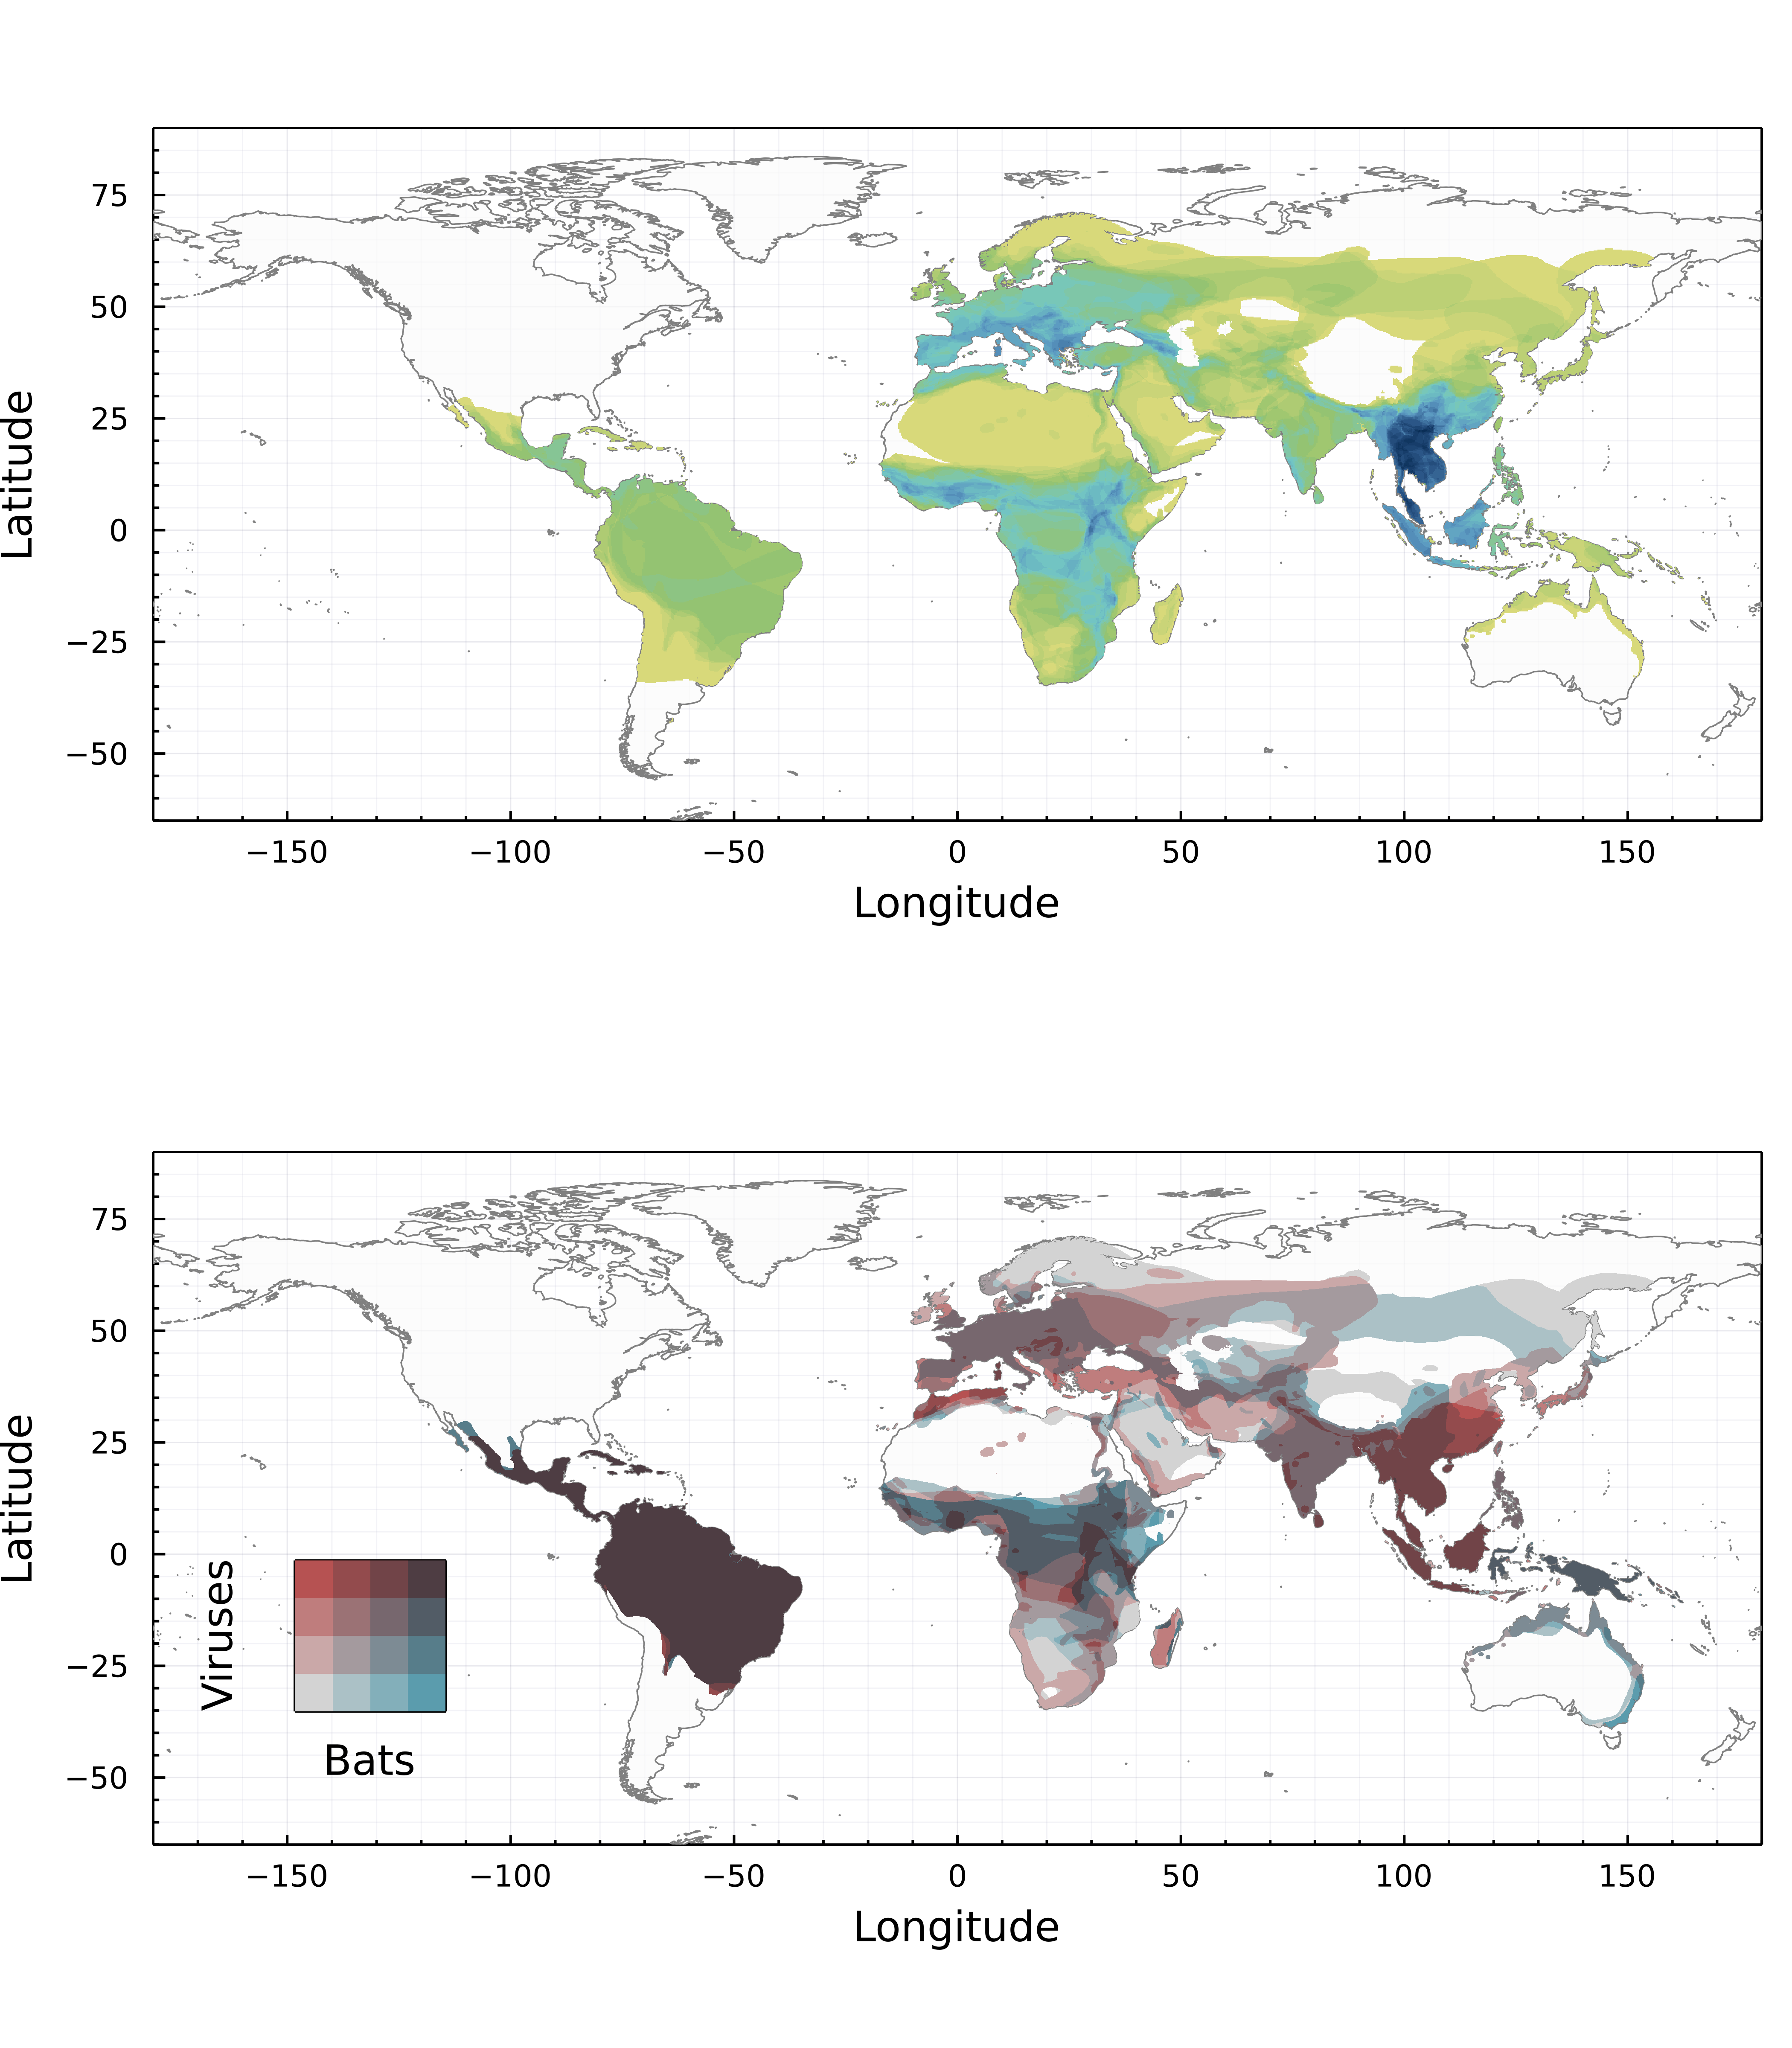
\includegraphics{figures/combined_richness.png}
\caption{Top panel: relative diversity of known bat hosts of
betacoronaviruses. This map shows that the region with the largest
number of possible hosts is South-Eastern Asia. Bottom panel: congruence
between the evolutionary distinctiveness of the hosts (grey to blue) and
the viruses (grey to red).}\label{fig:richness}
}
\end{figure}

However, we find that the global pattern of betacoronavirus phylogenetic
distinctiveness is quite distinct from both bat host richness and
phylogenetic distinctiveness (fig.~\ref{fig:richness}; bottom). In
contrast to the sparsity of Neotropical betacoronavirus hosts, South
America has the most evolutionary distinct hosts \emph{and} viruses,
followed by secondary hotspots in southeast Asia and the Rift Valley
region have mostly distinct viruses. Some degree of sampling bias may
contribute to these patterns: for example, South-America is one of the
places where the fewest bat betacoronavirus sequences have been
generated,\textsuperscript{2,13,15} resulting in a sparser phylogenetic
tree, and artificially inflating distinctiveness; conversely,
disproportionate research effort in eastern China\textsuperscript{16}
may have led to a more complete inventory of the local diversity of
coronaviruses, again inflating these metrics relative to underlying
patterns. Even accounting for these potential biases, though, there is
obvious heterogeneity in betacoronavirus evolutionary distinctiveness
that is distinct from overall bat diversity.

On closer inspection, these patterns recapitulate the evolutionary
history of both the order Chiroptera and the genus
\emph{Betacoronavirus}. Horseshoe bats (Rhinolophidae) are both the
reservoirs of the SARS-like viruses (subgenus \emph{Sarbecovirus}) and a
possible ancestral host of \emph{Betacoronavirus}.\textsuperscript{17}
The hotspots of host richness and viral diversity in southeast
Asia---both of which are disproportionately high, considering the global
landscape of bat species richness---are almost entirely driven by viral
adaptive radiation through host switching within this
clade\textsuperscript{3,14}. In contrast, the Neotropical hotspot of
viral distinctiveness is driven by isolation by host vicariance. Out of
the four main groups of betacoronaviruses, only the subgenus
\emph{Merbecovirus} (MERS-like viruses) has been found in animals in the
Americas---an introduction that is generally presumed to be
ancient.\textsuperscript{3} While comparatively understudied, New World
merbecoviruses have been found in the ghost-faced bats (Mormoopidae),
New World leaf-nosed bats (Phyllostomidae), and free-tailed bats
(Molossidae) (add cite: Olival 2020 PLoS Pathogens). The former two
groups are endemic to the Neotropics, while the explosive adaptive
radiations of the latter two (and particularly the phyllostomids) are
responsible for the hotspot of bat diversity in the Amazon. Together,
these clades of New World bats play host to a distinct regime of
betacoronavirus coevolution.

\hypertarget{global-biogeographic-regions-are-consistent-for-bats-and-betacoronaviruses}{%
\subsection{Global biogeographic regions are consistent for bats and
betacoronaviruses}\label{global-biogeographic-regions-are-consistent-for-bats-and-betacoronaviruses}}

Most previous work has assumed that coronavirus biogeography is driven
by coevolutionary regimes that form at finer taxonomic scales, treating
the presence or richness of key bat host groups as predictive of these
viruses' distribution.\textsuperscript{2,3} Projecting bat and
betacoronavirus phylogeny over space (fig.~\ref{fig:biogeo}), we find
further support for the idea that bat community assembly is directly
responsible for spatial heterogeneity in viral coevolutionary regimes.
The distinct groupings (represented by different colors, symbolizing
positions in a subspace formed by the first two phylogenetic principal
components) are essentially equivalent between the two groups, and can
be coarsely delineated as (1) south and southeast Asia, (2) east Asia
(including northern China), west Asia, and the Mediterranean coast; (3)
Eurasia above a northing of 40; and (4) Africa and south America. In
some cases, this diverges from expectations about coronavirus
biogeography: for example, previous work has rarely flagged India as a
region of concern, but for both bats and betacoronaviruses, the
subcontinent falls into the same phylogeographic regions as the
southeast Asian peninsula (and indeed, the region is home to known bat
hosts of nobecoviruses, sarbecoviruses, and
merbecoviruses).\textsuperscript{3}

\begin{figure}
\hypertarget{fig:biogeo}{%
\centering
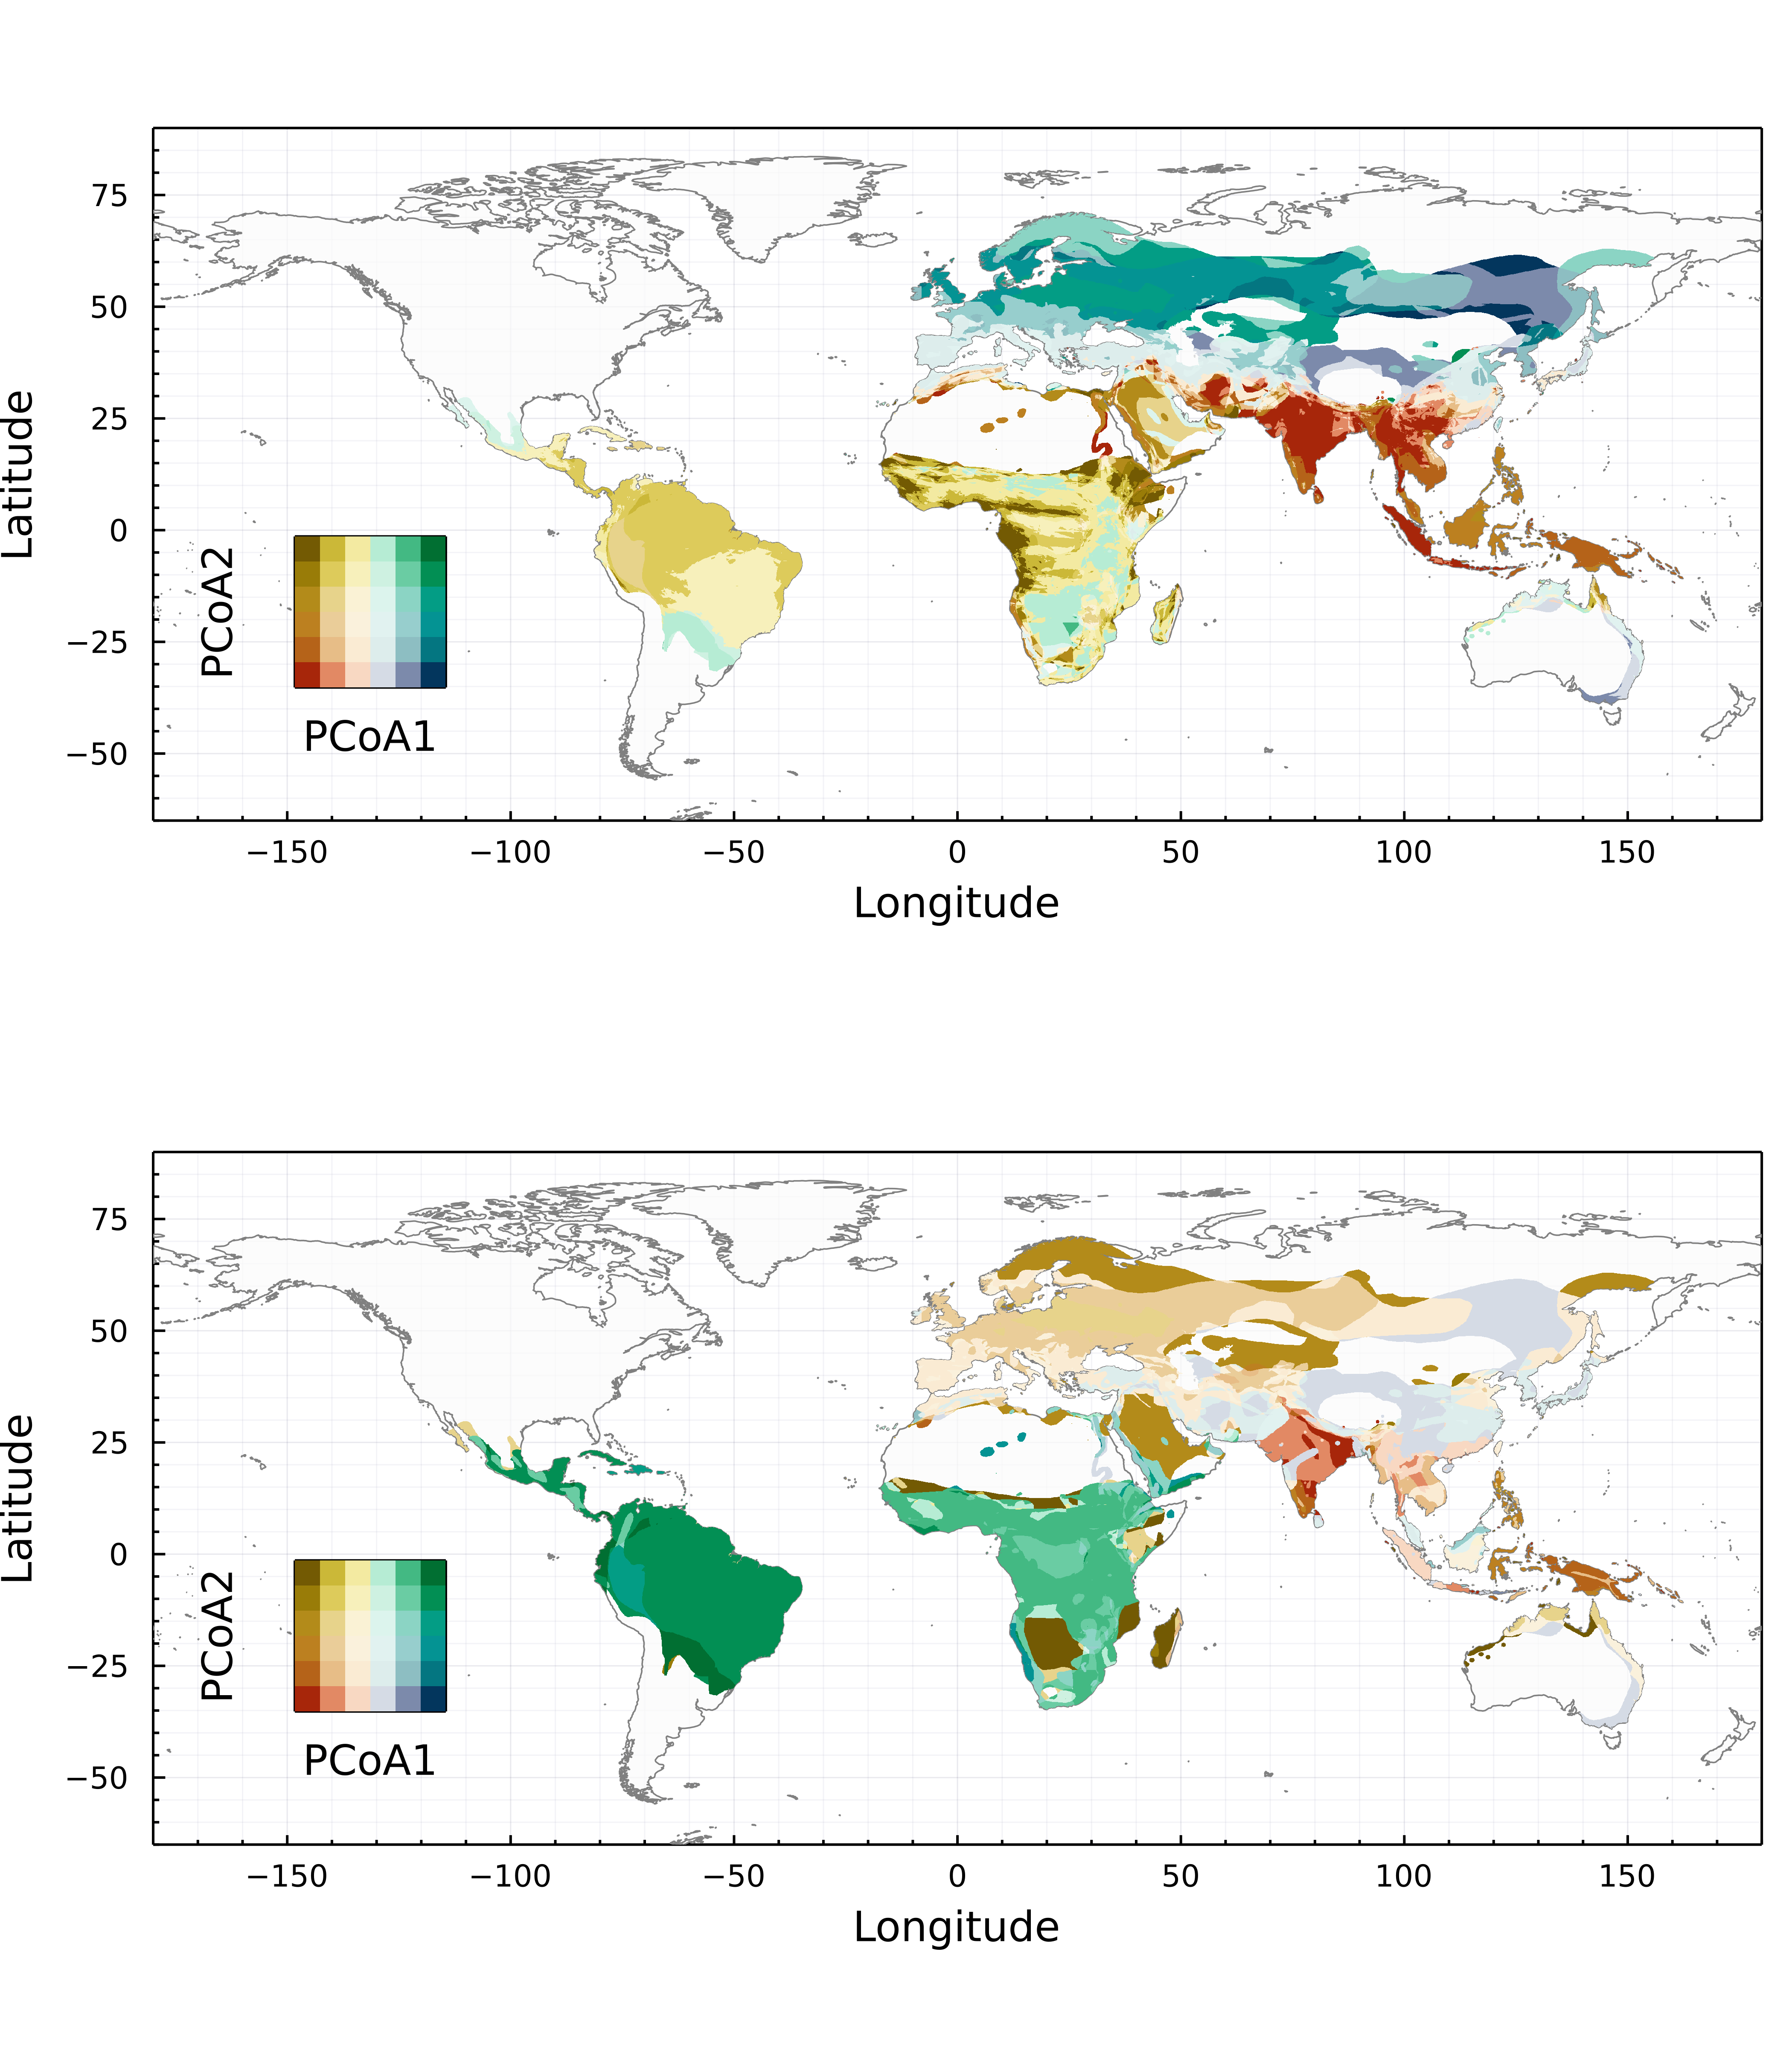
\includegraphics{figures/combined_biogeo.png}
\caption{Phylogeographic regions of bats (top) and viruses (bottom)
based on the joint analysis of their occurrence and phylogenetic
relatedness. The different colors show tendencies to separate alongside
the first two components of a PCoA. Note that the PCoA for the bats and
viruses are independent, and so cannot be compared directly -- that
being said, the regions can be compared across maps.}\label{fig:biogeo}
}
\end{figure}

Overall, these results suggest that, although there are unique hotspots
of viral adaptive radiation, biogeographic regions are mostly consistent
between bats and their viruses. This may be surprising, given that
cospeciation plays a minor role in coronavirus
diversification,\textsuperscript{2} which could theoretically allow for
broad divergence in their biogeography. However, host jumps at the
family level or higher are relatively rare and significant events in
coronavirus evolutionary history;\textsuperscript{2,17} as a result, we
suggest the mosaic of betacoronavirus phylogeography is assembled from a
set of overlapping smaller coevolutionary systems, superimposed in space
and filtered by the importance of different subgroups in local host
communities. For example, the most speciose and cosmopolitan family of
bats, the vesper bats (Vespertilionidae), are considered the primary
reservoir of merbecoviruses;\textsuperscript{3,17} but in the Americas,
where merbecoviruses are the only lineage present, they have only been
found in other bat taxa. At the coarsest scale, these heterogeneities
are lost, and betacoronavirus biogeography tracks the deep rifts in bat
evolutionary history---but within these broad regions, the component
coevolutionary systems can have very different dynamics.

\hypertarget{coevolution-informed-emergence-risk-is-different-in-space}{%
\subsection{Coevolution-informed emergence risk is different in
space}\label{coevolution-informed-emergence-risk-is-different-in-space}}

As host richness, joint distinctiveness, or phylogeographic structure
suggest that the bat-betacoronaviruses complex is globally fragmented
enough to give rise to both different levels of risk (as evidenced by
the spatial location of spillover events) and different types of
co-evolutionary dynamics, we turn to the Geographic Mosaic Theory of
Coevolution to provide a measure of risk accounting for multiple
processes. In fig.~\ref{fig:trivariate}, we overlapped three components
of spillover risk: viral sharing, \emph{i.e.} the chance that two bats
will share viruses overall; Local Contribution to Beta Diversity,
\emph{i.e.} the fact that a bat community is compositionally unique
compared to the average compositional similarity across the entire
system; finally, host phylogenetic diversity, \emph{i.e.} how dispersed
the bats in a location are within the tree of life. This approach leads
to the definition of broad biogeographic regions of risk, where the same
color represents the same type of risk. By way of constrat to figures
fig.~\ref{fig:richness} and fig.~\ref{fig:biogeo}, these regions do not
necessarilly overlap with previous spatial partitions of the
bat-betacoronaviruses complex.

\begin{figure}
\hypertarget{fig:trivariate}{%
\centering
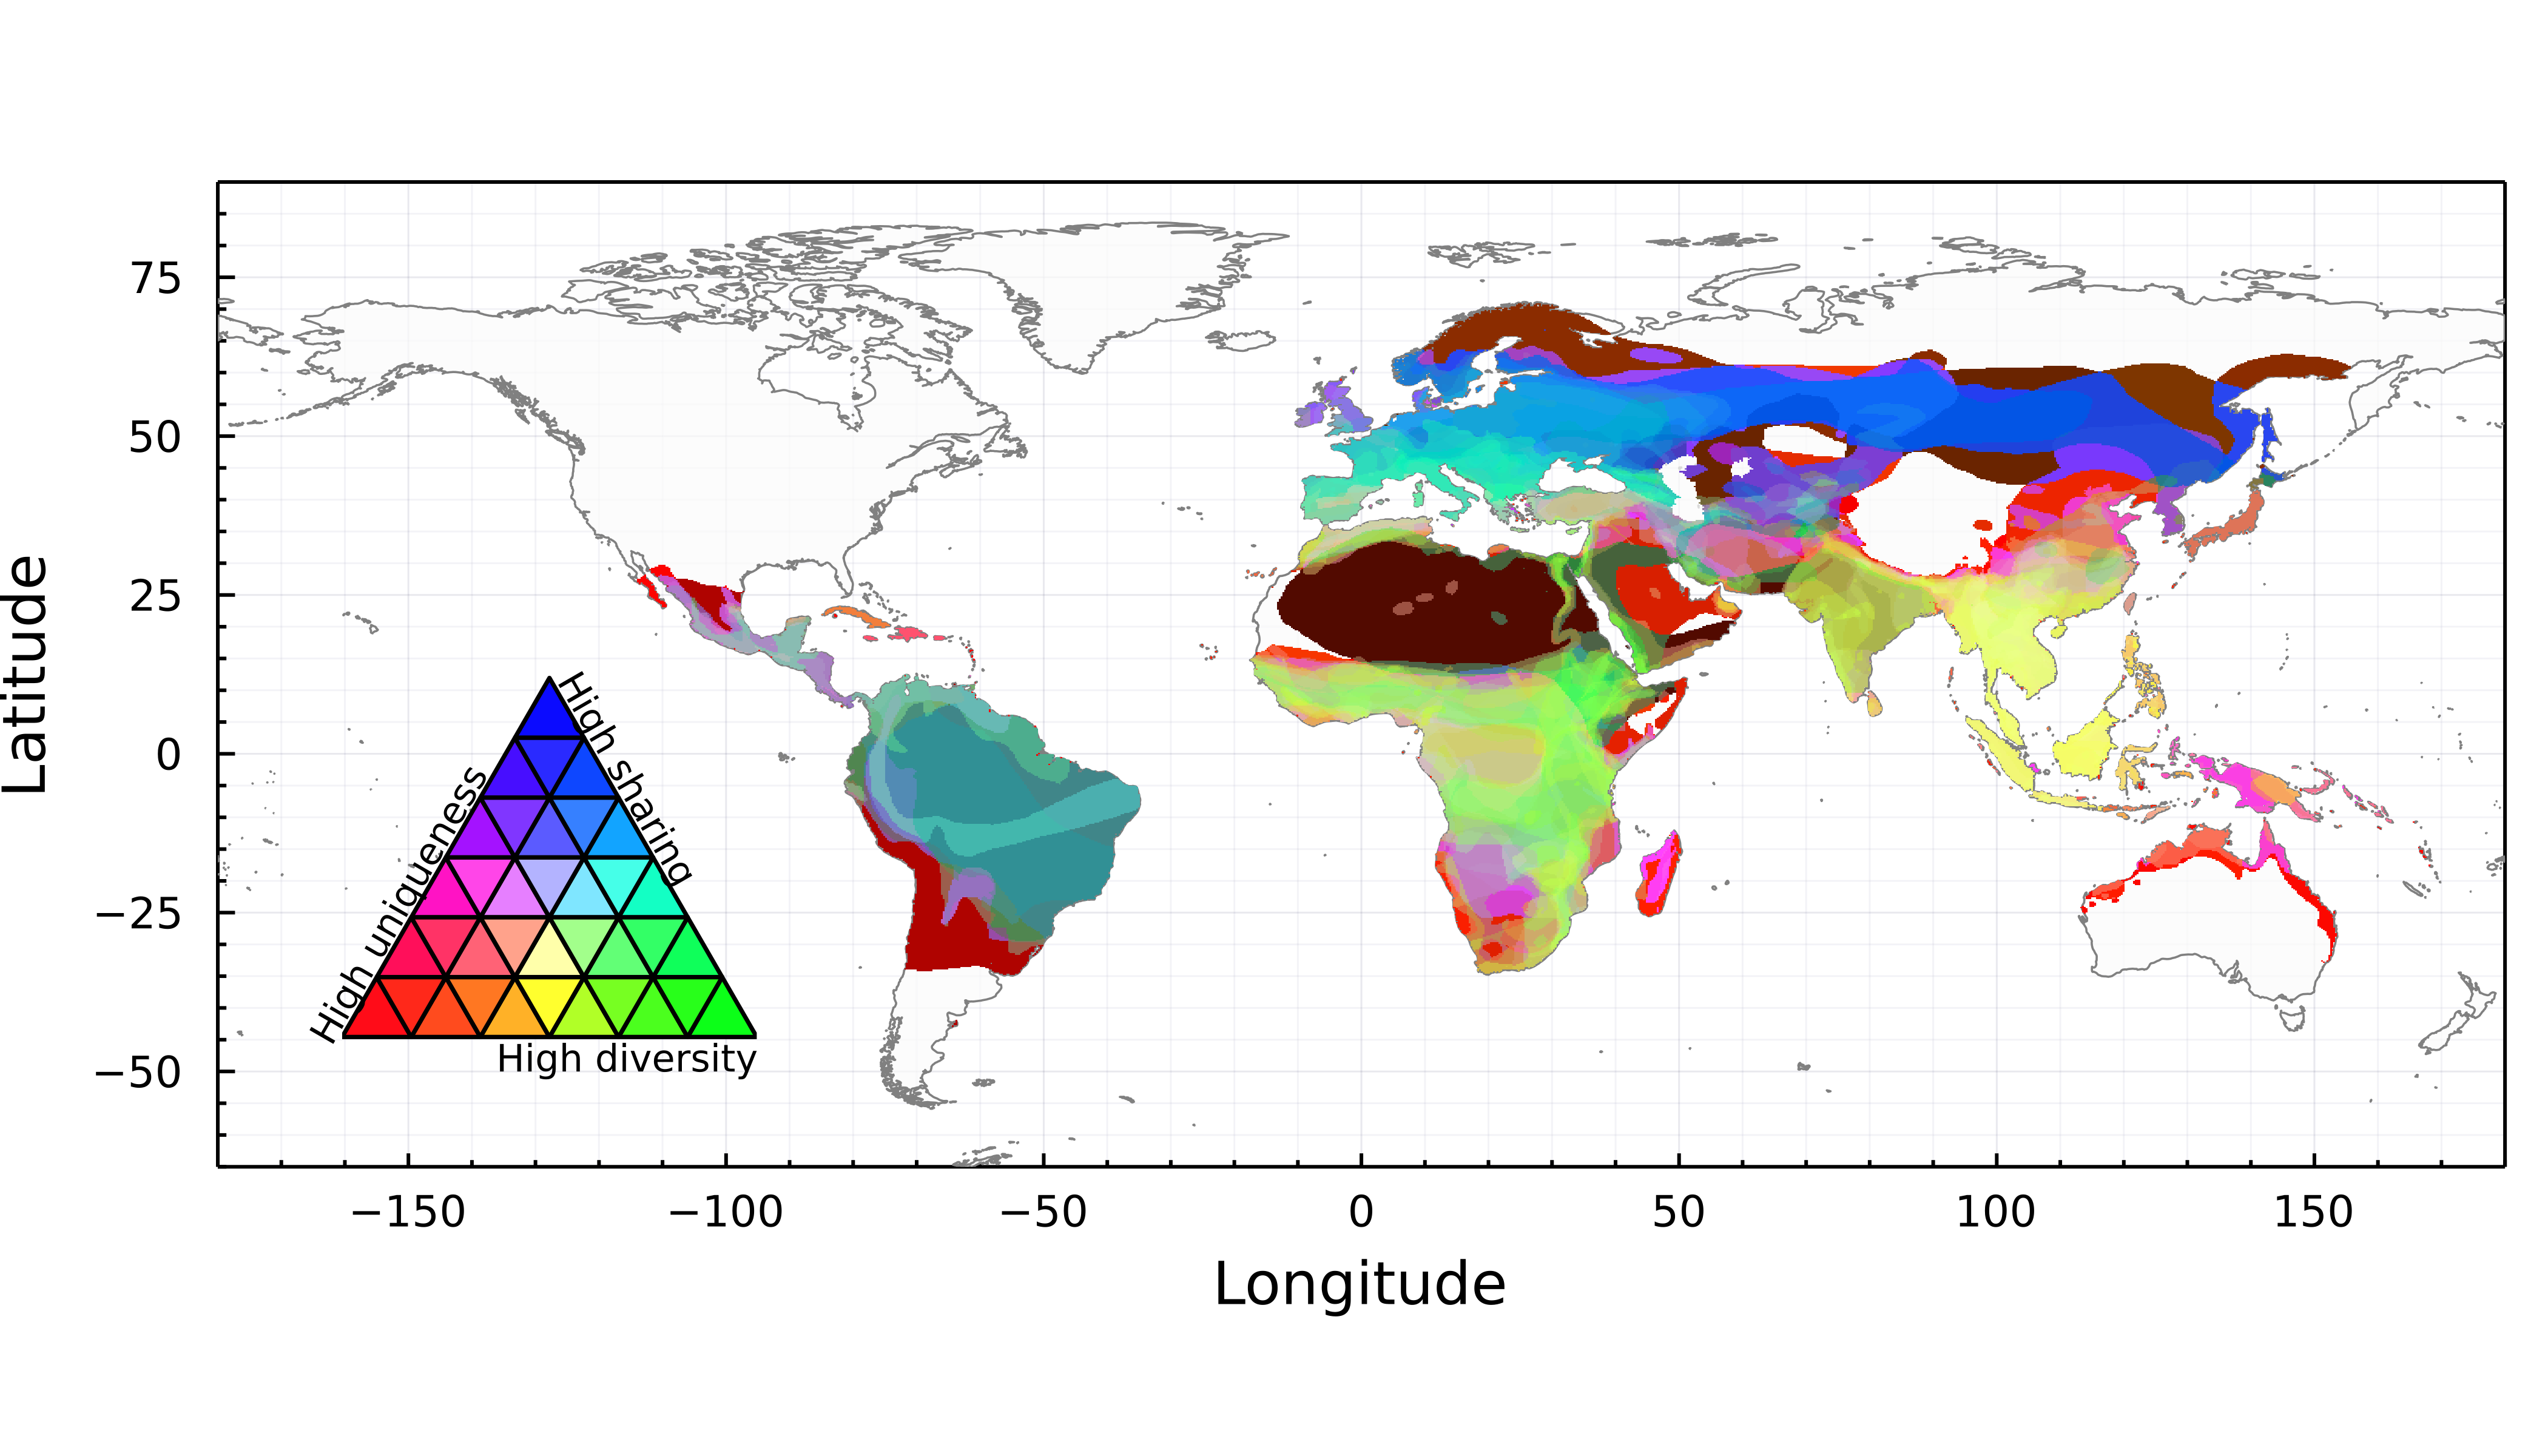
\includegraphics{figures/risk_trivariate.png}
\caption{Trivariate additive mapping of the components of risk in the
red/green/blue, where high virus sharing is encoded in the blue channel,
host phylogenetic diversity in the green channel, and compositional
uniqueness in the red channel. A pixel that would maximize all measures
(highest possible risk) would be a pure white (specifically RGB(1.0,
1.0. 1.0)), and a pixel with the lowest possible values would be pure
black (specifically RGB(0.0, 0.0, 0.0)). Therefore, lighter values (the
sum of the three channels gets closer to 3) indicate higher risk, and
the color indicates the proportional distribution of the factors making
up the total risk.}\label{fig:trivariate}
}
\end{figure}

From the perspective of spillover risk, the most important combination
of factors is a high phylogenetic diversity of hosts with low viral
sharing; this, essentially, means that very different betacoronaviruses
could co-exist within the same place. This is particularly the case
given that betacoronaviruses often evolve and even achieve host shifts
through recombination, which requires the co-occurrence of sufficiently
distinct viruses to be a major driver of emergence. In
fig.~\ref{fig:trivariate}, this corresponds to yellow to pale green
areas, which are essentially limited to South-Eastern Asia, and to some
part of Sub-Saharan Africa. Adopting a geographic mosaic theory
perspective on risk, other regions of the world are of lesser concern
(fig.~\ref{fig:risk}). Our risk decomposition does not account for viral
diversity or distinctiveness. The simple rationale behind it is that the
acquisition of viral data is rarely disconnected from the acquisition of
host data. There are more sources of information on hosts than on
viruses, allowing to develop a host-centric perspective on risk
(although this estimate would more accurate with viral traits related to
\emph{e.g.} ability to switch hosts or pathogenic potential). Areas with
high bat diversity and high turnover \emph{may} facilitate the
evolutionary radiation of viruses, matching previous findings that the
diversification of bat coronaviruses is driven largely by host shifts
(inter-genus or higher levels of cross-species transmission) and, to a
lesser degree, cospeciation and sharing, representing intra-genus
cross-species transmission.\textsuperscript{2} This diversification is
not an actual risk factor for spillover itself, but acts downstream of a
spillover event by increasing the random chance of the emergence of a
virus with the raw genomic components required for the potential to
infect humans.

\begin{figure}
\hypertarget{fig:risk}{%
\centering
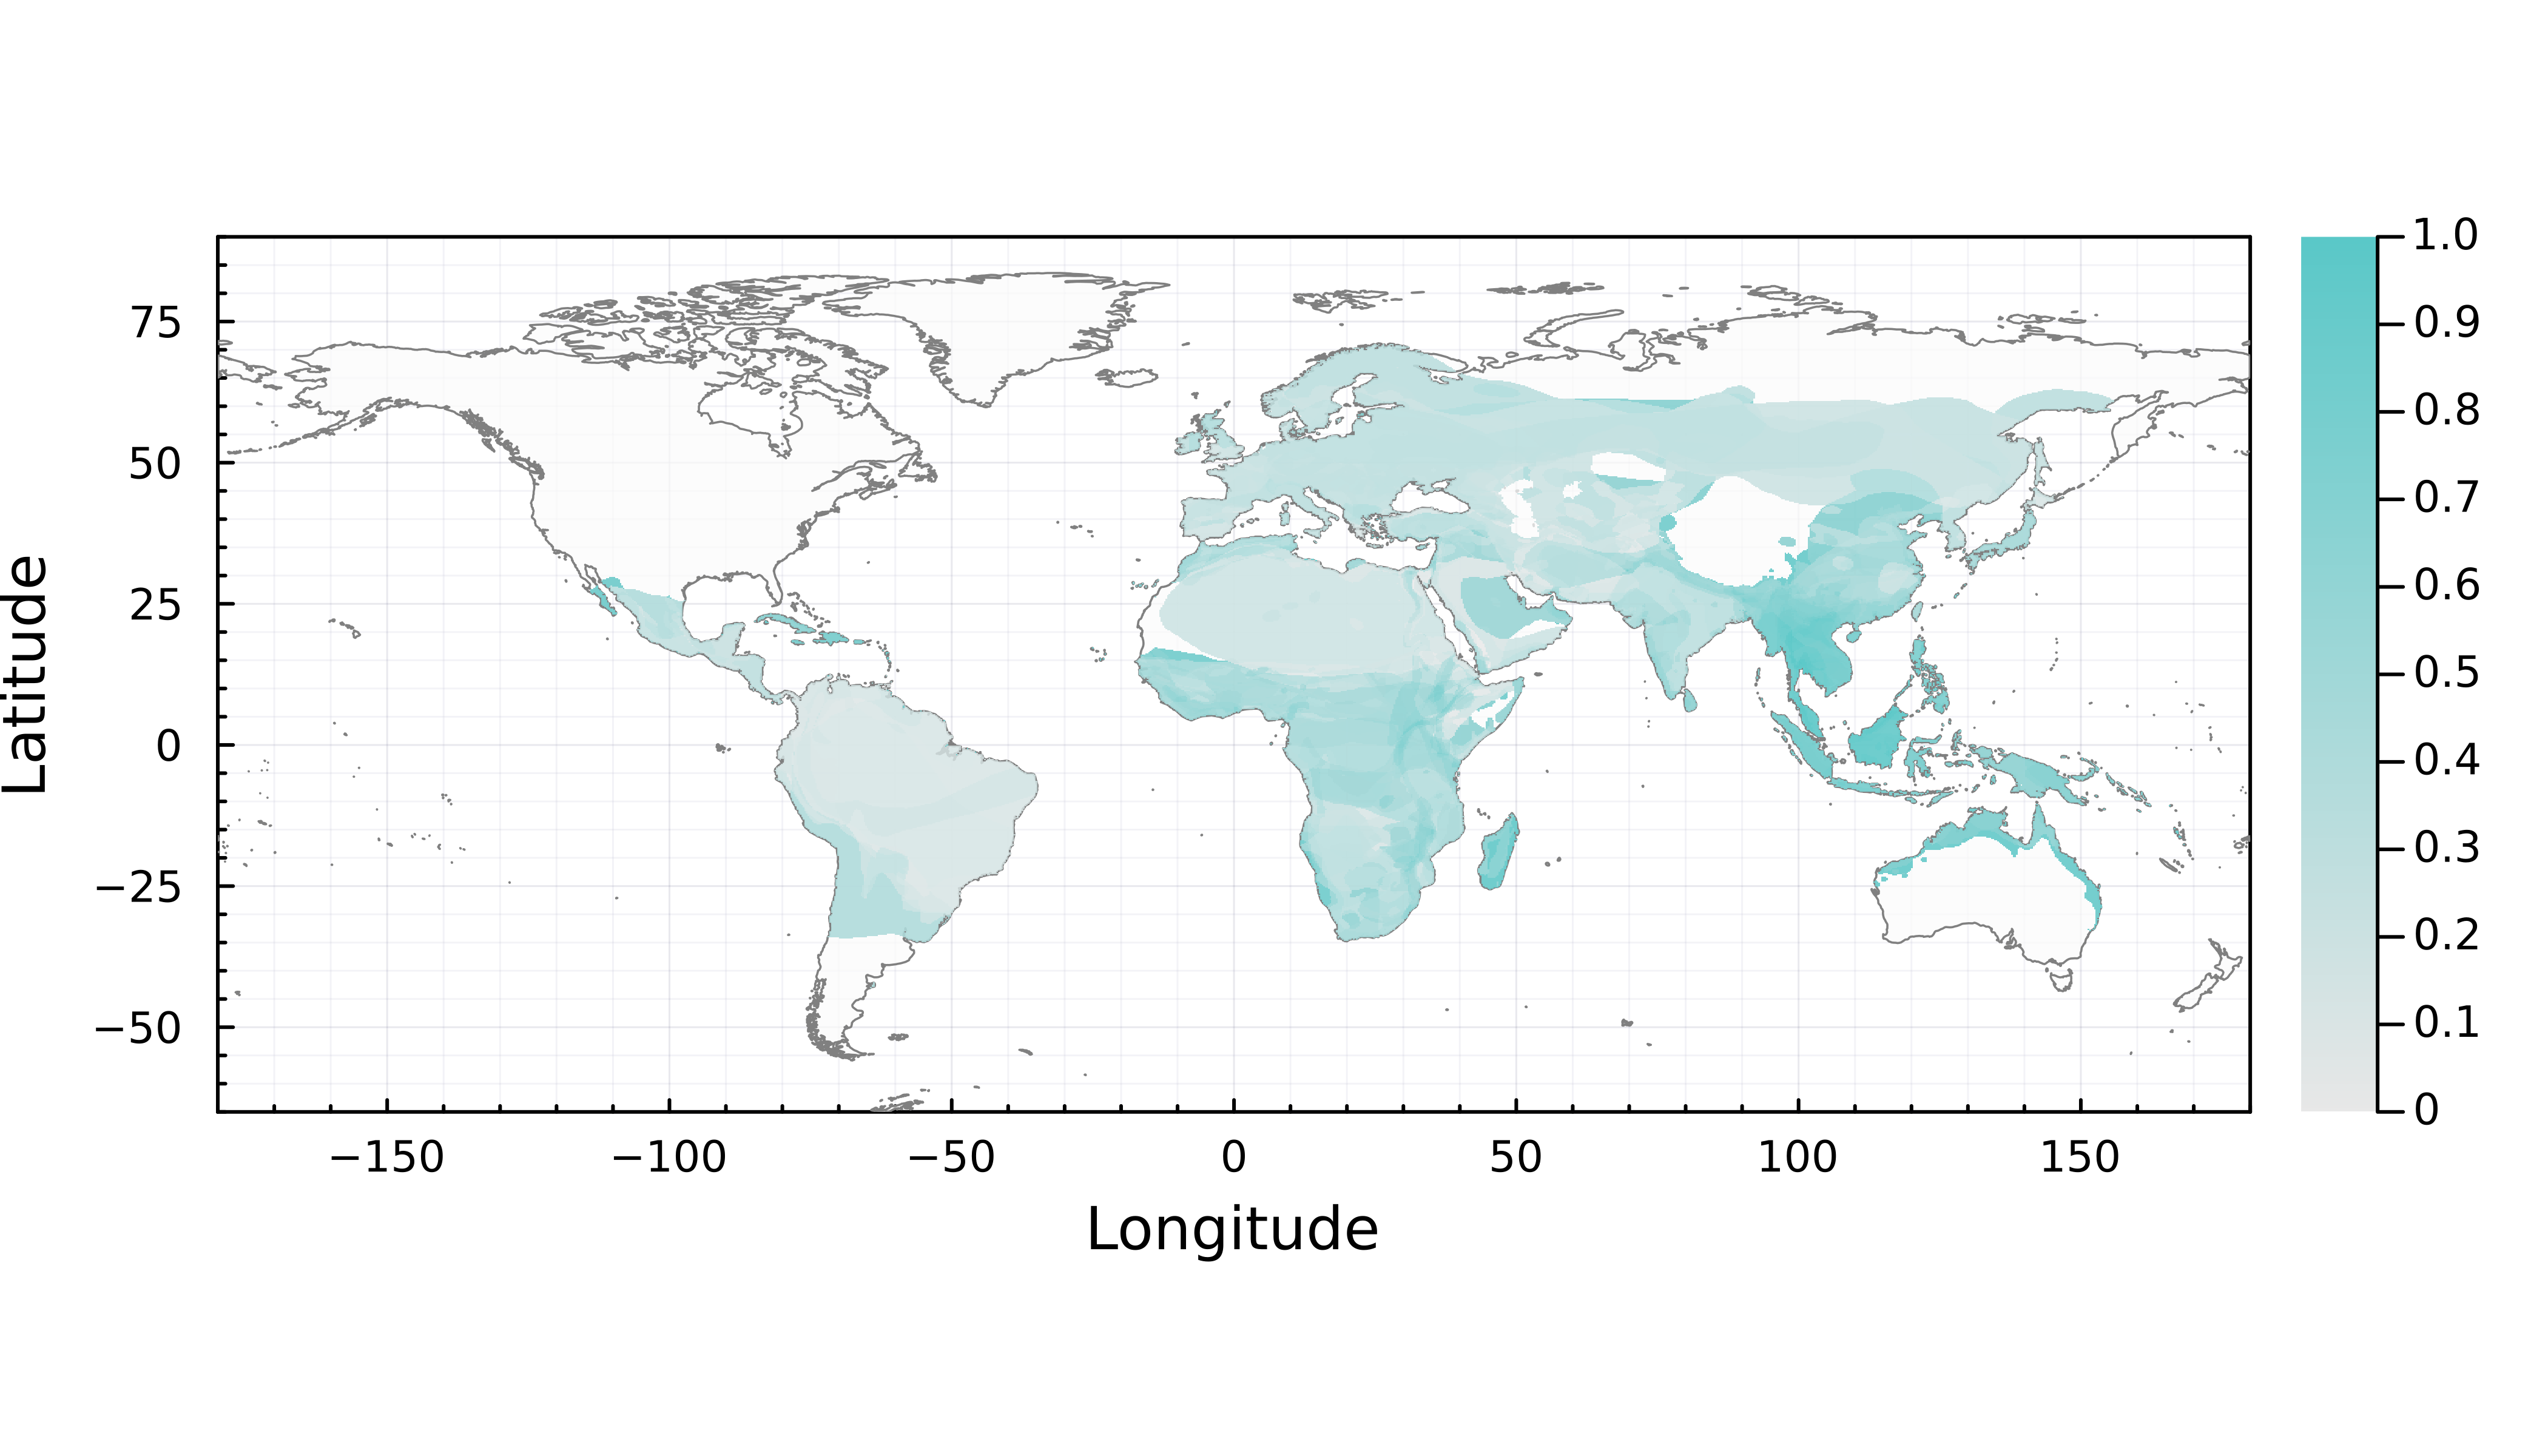
\includegraphics{figures/risk_map.png}
\caption{Extraction of a measure of \emph{Betacoronavirus} spillover
risk from bat hosts based on the colorimetric space from
fig.~\ref{fig:trivariate}. The risk is a composite measure of the color
value and angular distance to the yellow hue, as defined in the methods,
ranged in the unit space. Based on this analyses, regions at high risk
of spillover are southeast Asia and Madagascar.}\label{fig:risk}
}
\end{figure}

From another perspective, areas of high host uniqueness and virus
sharing (red-to-pink) could provide hotspots of \emph{Betacoronavirus}
risk through mixing of unique viruses (via codivergence) and in turn
recombination. Under our framework, such a hotspot was identified in
Madagascar, where most bat species are endemic following evolutionary
divergence from sister species in both African and Asian
continents.\textsuperscript{18} Recent surveillance\textsuperscript{19}
has identified a novel \emph{Betacoronavirus} (in the subgenus
\emph{Nobecovirus}) in Madagascar-endemic pteropid bat species
(\emph{Pteropus rufus}, \emph{Rousettus madagascariensis}), emphasizing
strong proof of principle in model predictions.

\hypertarget{human-occupancy-drives-different-levels-of-effective-risk-globally}{%
\subsection{Human occupancy drives different levels of effective risk
globally}\label{human-occupancy-drives-different-levels-of-effective-risk-globally}}

Based on the previous result, we extracted the risk component from the
composite map (see Methods), to provide a single measure of risk varying
between 0 and 1. This measure is presented in fig.~\ref{fig:risk}. As
this map represents the potential risk, it must be weighed by the
potential for contacts with humans. As a proxy for this measure, we used
the proportion of build/urban land from the EarthEnv dataset: this is a
reasonable proxy for the density of humans per unit area, which
increases the probability of pathogen spread more
widely.\textsuperscript{20} Since human activity is required to amplify
the frequency of virus encounters and thus create areas of viral
amplification, mapping the potential risk against measures of land use
is required to generate a more actionable assessment of risk. This map
is presented in fig.~\ref{fig:compound}. Most of South America and
Europe are at comparatively lower risk, as although densely populated,
settlements tend to be in areas with lower potential risk. Regions like
Malaysia and the North coast of Australia have a high risk component,
but should represent a relatively lower effective risk due to low human
density. However, this mapping reveals that South-East Asia, the Indian
subcontinent, and parts of sub-Saharan Africa, are at high risk due to
the overlap between built areas and bat communities representing more
opportunities for cross-species transmission of betacoronaviruses. In
looking for the origins of SARS in China,\textsuperscript{21} present
serological evidence that strongest human-animal contact results in
higher risk of virus exposure, regardless of the animal species, but
that different types of contact had different impacts. Ideally,
finer-grained information about human activity (rather than human
presence through anthropisation) could allow to partition this risk
further, alebit at the cost of more hypotheses required to estimate the
amount of risk represented by each activity. Our map of purported high
risk/diversitifcation potential (Madagascar, South-America) overlay with
sampling gaps for \emph{Betacoronavirus},\textsuperscript{16} stressing
the need for spatially targeted monitoring and discovery.

\begin{figure}
\hypertarget{fig:compound}{%
\centering
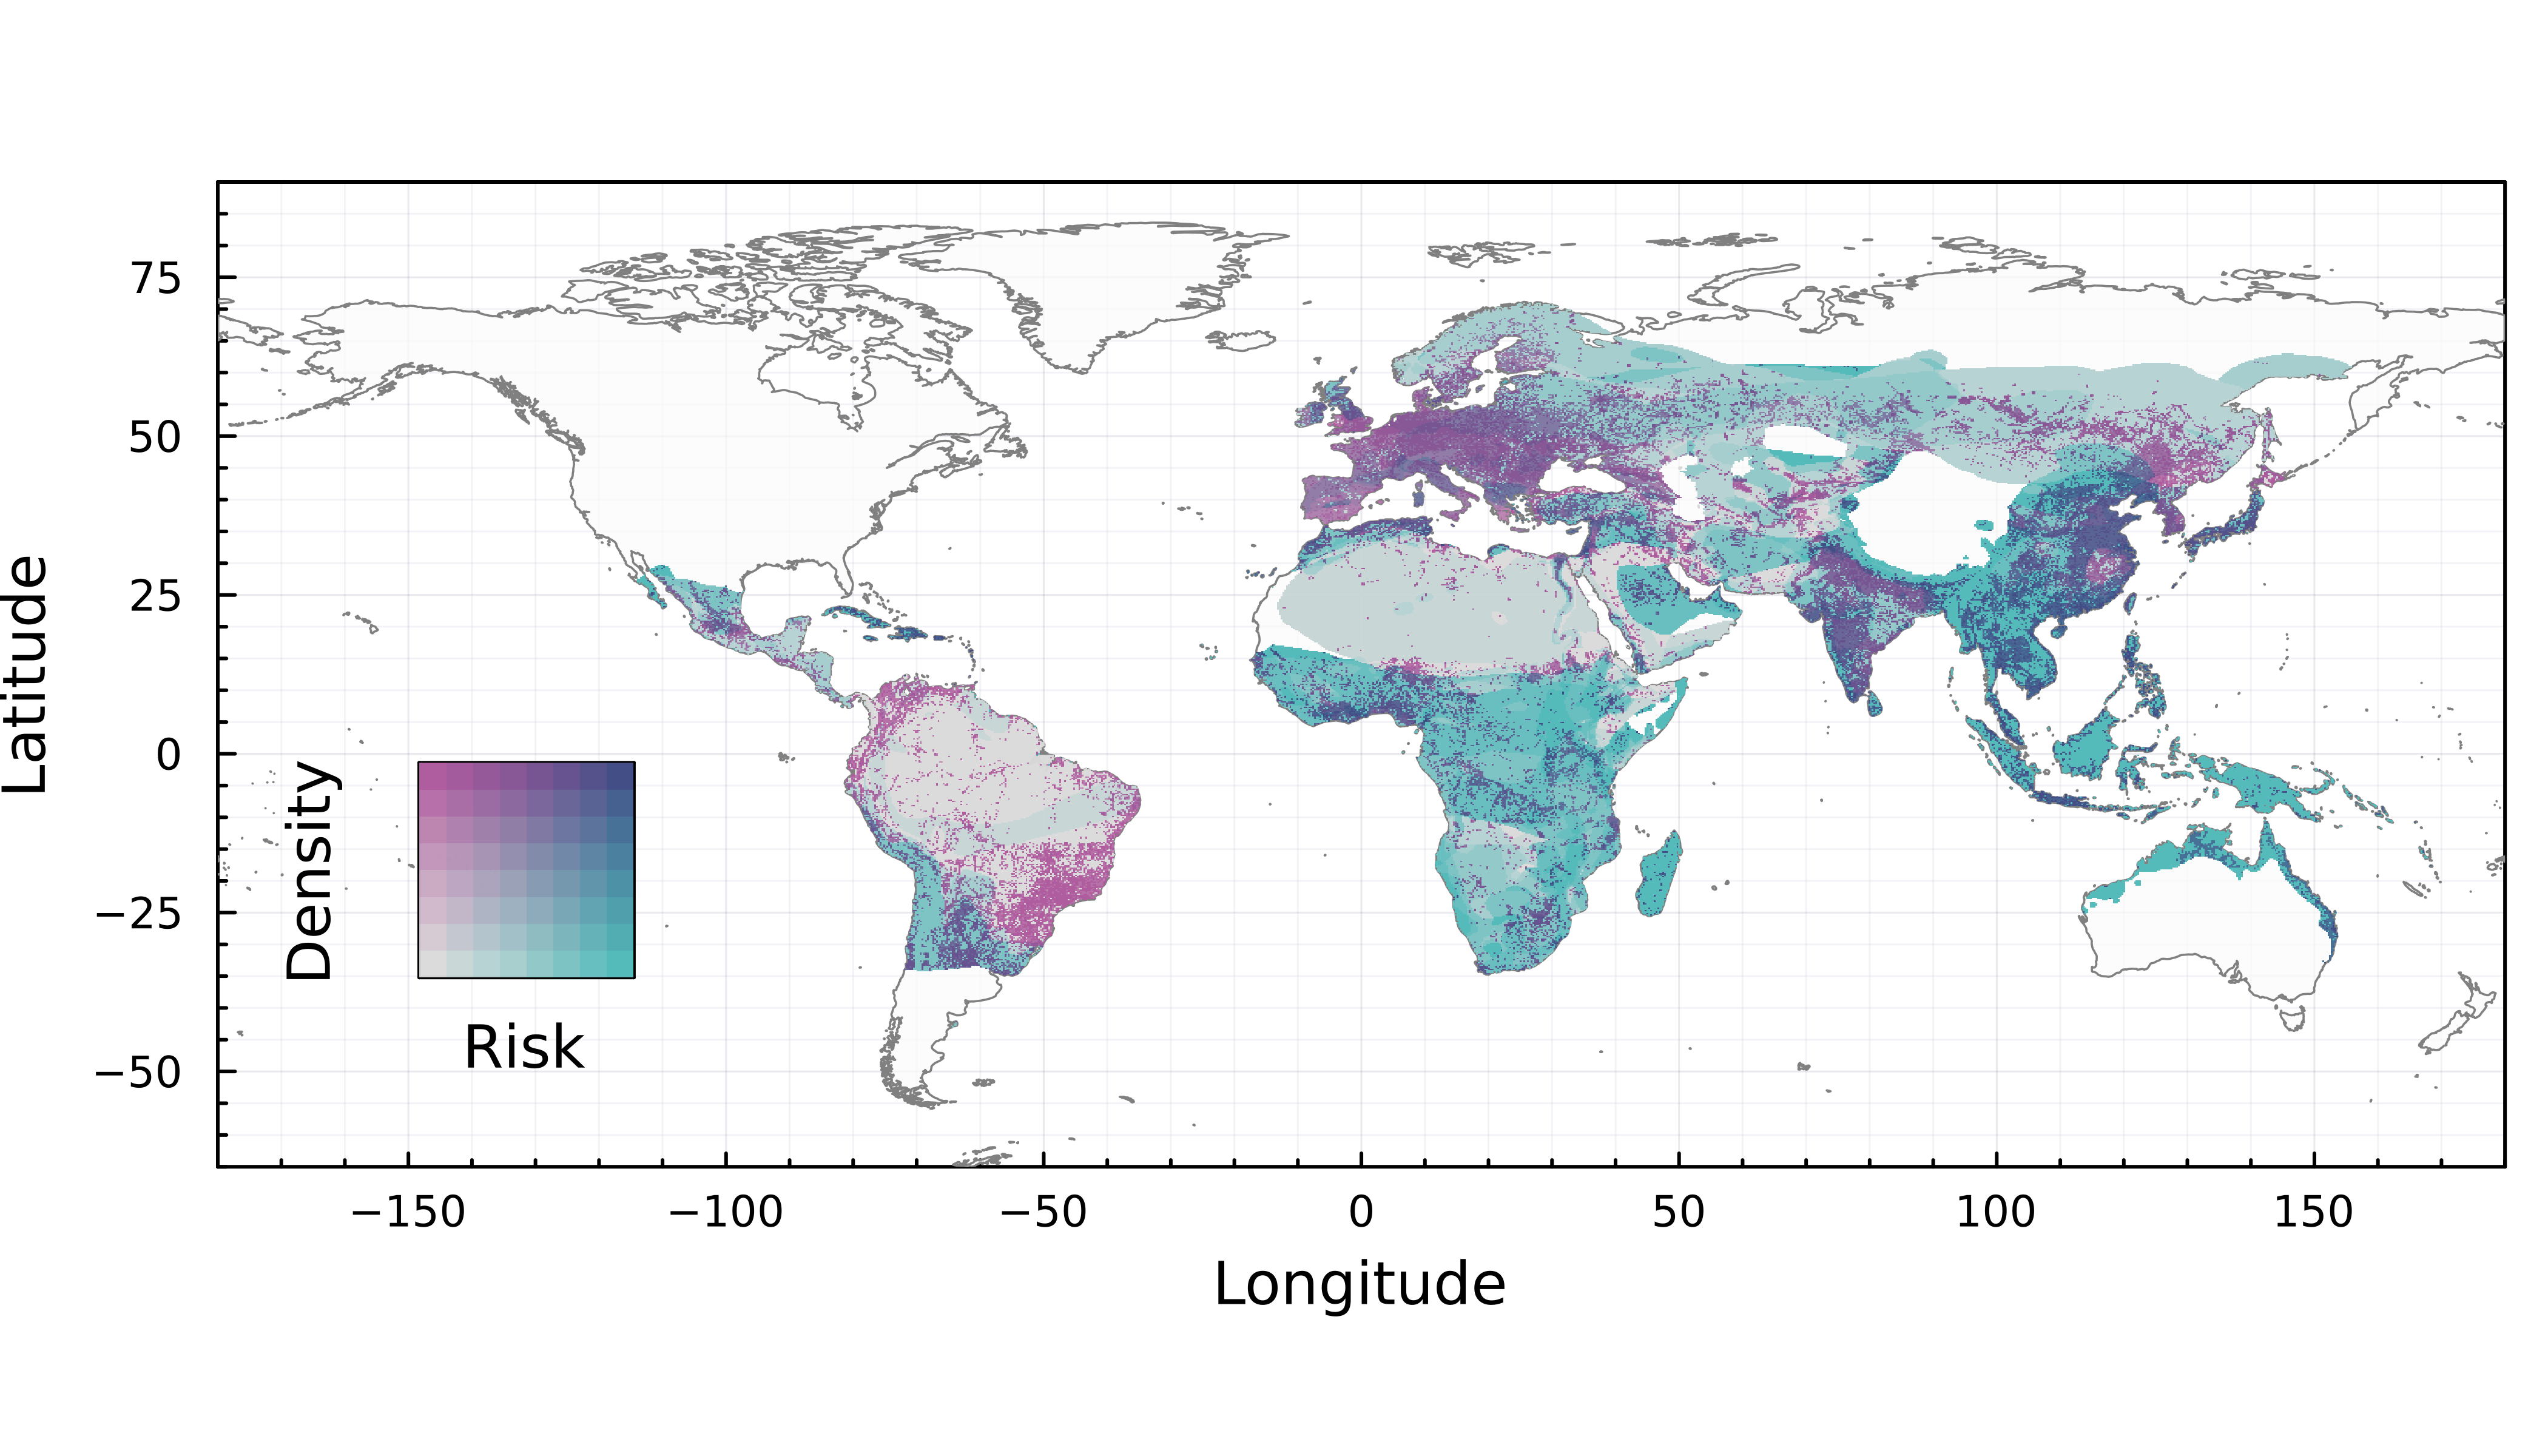
\includegraphics{figures/risk_compounded.png}
\caption{Overlap of the percent of each pixel occupied by urbanized
structures, representing the degree of settlement, on the spillover risk
map (where the risk comes only from wildlife, and ignores multi-hosts
chains of transmissions including non-bats hosts). Darker pixels
correspond to more risk, in that the GMTC-derived risk of
fig.~\ref{fig:risk} is high \emph{and} the pixel is densely occupied by
human populations. This approach increases the relative risk of several
regions in Africa, and highlights the risk in India, southeast China,
and the Arabian peninsula where areas of high to moderate risk overlap
with areas of denser population.}\label{fig:compound}
}
\end{figure}

PUT THIS SOMEWHERE: Available information describing the spillover of
zoonotic betacoronaviruses of bat origin where data was available before
and up through the COVID-19 pandemic puts spillover events of SARS-CoV-2
in Wuhan, China; SARS-CoV in Guangdong, China based on the presence of
closest known viruses circulating in nature, and a nearby location where
serological (antibody) evidence has indicated human exposure to
SARS-like viruses;\textsuperscript{22} MERS-CoV in Saudi Arabia based on
index cases available from a recently-published compendium of
cases.\textsuperscript{23} For the latest event, most if not all index
cases are presumed to be camel-to-human transmission, and the precise
origin point (if it exists) of MERS-CoV in bats is uncertain. Recent
recombinant canine coronavirus spillover events in
Haiti\textsuperscript{24} and Europe\textsuperscript{25} are not
relevant here, as bats' involvement in these cycles of transmission have
been supposed to be non-existent. These index cases fall within
different phylogeographic bioregions (fig.~\ref{fig:biogeo}), which
further highlight the issue that different host-virus sub-systems may
lead to widespread emergence.

\hypertarget{conclusion}{%
\section{Conclusion}\label{conclusion}}

Bats are important reservoir hosts for different classes of
microorganisms, many of which a threat to human
health.\textsuperscript{26,27} Chiropterans emerged around 64 million
years ago and are one of the most diverse mammalian orders, with an
estimated richness of more than 1400 species.\textsuperscript{28,29}
They exhibit a broad variety of habitat use, behaviour, and feeding
strategies, putting them at key positions in the delivery and
provisioning of several ecosystem services, tied to important
ecosystem-derived benefits to human.\textsuperscript{30} For example,
bats are an essential component of many seed-dispersal
networks.\textsuperscript{31} Over two-thirds of bats are know to be
either obligate or facultative insectivores, therefore actively
contributing for agricultural pest control,\textsuperscript{32,33} and
vectors of pathogens that put a risk on human
health.\textsuperscript{34,35} Because bats are globally distributed and
have a long evolutionary history, phylogeographic and biogeographic
approaches are required to shed light on the contemporary distribution
of coevolutionary processes between bats and the pathogens they host.
Not all areas in which bats, viruses, and human are co-occuring are
facing a risk of spillover towards human populations, and the areas in
which this risk exist may not be facing risks of the same nature and
magnitude.

Here, we propose a simple freamework with broad explanatory power that
helps contextualize discoveries like highly divergent nobecoviruses in
Madagascar and the previously-neglected adaptive radiation of
sarbecoviruses outside of southern China and throughout southeast Asia.
In doing so, it advances ecological theory beyond the current state of
the art for global maps of emergence risk. For example, previous studies
that have used host richness as proxy have predicted a high diversity of
unsampled bat viruses,\textsuperscript{13} bat
coronaviruses,\textsuperscript{2} and even specifically
betacoronaviruses\textsuperscript{14} in both the Amazon and southeast
Asia. While we find that both regions are characterized by highly
divergent host and viral communities, our framework identifies key
differences between the regions. We find that Latin America is a hotspot
of both host and viral distinctiveness, suggesting that this branch of
the bat-betacoronavirus complex may be undergoing independent
evolutionary dynamics from the rest of the global pool, but with limited
potential for viral diversification--- a finding that is supported by
previous work indicating a higher rate of codivergence in Latin
America.\textsuperscript{2} In contrast, in southeast Asia, host
richness and viral distinctiveness are high but sharing is low; this
suggests a different type of evolutionary dynamics that could generate
high local diversity of viruses through host switching and viral
recombination (see \emph{e.g.},\textsuperscript{17} as well as the
discovery of recombinant viruses that share genetic material from both
the SARS-CoV and SARS-CoV-2 branches of the Sarbecovirus
lineage).\textsuperscript{36} Both of these regions are priority areas
for sampling, especially given predictions that they contain many bat
hosts of undiscovered betacoronaviruses.\textsuperscript{14,16} However,
both the evolutionary and ecological aspects of emergence risk are
likely higher in southeast Asia---a fact that will only become more
relevant, as bats track shifting climates and exchange viruses with
other species, creating a hotspot of cross-species transmission unique
to the region.\textsuperscript{37}

The diversity and diversification potential of bats responds to
anthropogenic factors others than shifting climates.\textsuperscript{38}
Land use changes could significantly decrease bat suitability, notably
through effects on diet and availability of
habitats.\textsuperscript{39} As our results establish that the
diversification of bats betacoronaviruses happens on top of processes
affecting hosts, biogeographic variation in human population density and
anthropogenic disturbances may feed into co-evolutionary dynamics.
Increase in humans-hosts contacts also increase the risk of emergence of
novel diseases,\textsuperscript{40} so does the changes in landscape
connectivity at local/regional scales.\textsuperscript{41} This
represents a challenge for both conservation strategies and disease
ecology: some areas can a high emergence risk and more potential for the
acquisition of zoonotic viruses through bat-human
encounters.\textsuperscript{42} In particular, the challenge ahead lies
in the need to quantify actual exposure (and risk) accounting for
several transmission scenarios, including both direct and indirect bat -
human interactions, and feeding back into the provision of ecosystem
services by bats.

\textbf{Acknowledgements}: We acknowledge that this study was conducted
on land within the traditional unceded territory of the Saint Lawrence
Iroquoian, Anishinabewaki, Mohawk, Huron-Wendat, and Omàmiwininiwak
nations. This work was supported by funding to the Viral Emergence
Research Initiative (VERENA) consortium including NSF BII 2021909 and a
grant from Institut de Valorisation des Données (IVADO). This research
was enabled in part by support provided by Calcul Québec
(www.calculquebec.ca) and Compute Canada (www.computecanada.ca). NF is
funded by the NSERC BIOS² CREATE program. TP and NF are funded by the
Courtois Foundation. RLM was supported by Bryce Carmine and Anne Carmine
(née Percival), through the Massey University Foundation. DJB was
supported by the National Institute of General Medical Sciences of the
National Institutes of Health (P20GM134973).

\newpage

\hypertarget{methods}{%
\section{Methods}\label{methods}}

\hypertarget{known-betacoronavirus-hosts}{%
\subsection{\texorpdfstring{Known \emph{Betacoronavirus}
hosts}{Known Betacoronavirus hosts}}\label{known-betacoronavirus-hosts}}

We downloaded the data on bats hosts of \emph{Betacoronavirus} from
\texttt{https://www.viralemergence.org/betacov} on
Apr.~2022,\textsuperscript{14} and filtered it to ``known'' hosts
(established before the emergence of SARS-CoV-2) and ``novel'' hosts
(confirmed through sampling and competence assays since the initial data
collection). The original database was assembled by a combination of
data mining and literature surveys, including automated alerts on the
``bats'' and ``coronavirus'' keywords to identify novel empirical
evidence of bats-betacoronaviruses associations; this yielded a total of
126 known hosts, 47 of which were novel hosts.

\hypertarget{bat-occurrences}{%
\subsection{Bat occurrences}\label{bat-occurrences}}

We downloaded the rangemap of every current bat species that was
classified as an empirically documented host of \emph{Betacoronavirus}
from the previous step, according to recent IUCN
data.\textsuperscript{43} The range maps were subsequently rasterized
using the \texttt{rasterize} function from
\texttt{GDAL}\textsuperscript{44} at a resolution of approximately
100kmx100km. For every pixel in the resulting raster where at least one
bat host of \emph{Betacoronavirus} was present, we extract the species
pool (list of all known bat hosts), which was used to calculate the
following risk assessment components: bat phylogenetic diversity, bat
compositional uniqueness, and predicted viral sharing risk.

\hypertarget{bat-phylogenetic-diversity}{%
\subsection{Bat phylogenetic
diversity}\label{bat-phylogenetic-diversity}}

For every pixel, we measured Faith's Phylogenetic
Diversity\textsuperscript{45} based on a recent synthetic tree with
robust time calibration, covering about 6000 mammalian
species.\textsuperscript{46} Faith's PD measures the sum of unique
branches from an arbitrary root to a set of tips, and comparatively
larger values indicate a more phylogenetic diverse species pool. We
measured phylogenetic diversity starting from the root of the entire
tree (and not from Chiroptera); this bears no consequences on the
resulting values, since all branches leading up to Chiroptera are only
counted one per species pool, and (as we explain when describing the
assembly of the composite risk map), all individual risk components are
ranged in {[}0,1{]}. This measure incorporates a richness component,
which we chose not to correct for; the interpretation of the
phylogenetic diversity is therefore a weighted species richness, that
accounts for phylogenetic over/under-dispersal in some places.

\hypertarget{bat-compositional-uniqueness}{%
\subsection{Bat compositional
uniqueness}\label{bat-compositional-uniqueness}}

For every species pool, we measured its Local Contribution to
Beta-Diversity;\textsuperscript{47} LCBD works from a species-data
matrix (traditionally noted as \(\mathbf{Y}\)), where species are rows
and sites are columns, and a value of 1 indicates occurrence. We
extracted the Y matrix assuming that every pixel represents a unique
location, and following best practices\textsuperscript{48} transformed
it using Hellinger's distance to account for unequal bat richness at
different pixels. The correction of raw community data is particularly
important for two reasons: first, it prevents the artifact of richer
sites having higher importance; second, it removes the effect of overall
species richness, which is already incorporated in the phylogenetic
diversity component. High values of LCBD indicate that the pixel has a
community that is on average more dissimilar in species composition than
what is expected knowing the entire matrix, i.e.~a more unique
community. Recent results by\textsuperscript{49} shows that LCBD
measures are robust with regards to spatial scale, and are therefore
applicable at the global scale.

\hypertarget{viral-sharing-between-hosts}{%
\subsection{Viral sharing between
hosts}\label{viral-sharing-between-hosts}}

For all bat hosts of \emph{Betacoronavirus}, we extracted their
predicted viral sharing network, generated from a previously published
generalized additive mixed model of virus sharing by a tensor function
of phylogenetic distance and geographic range overlap across
mammals.\textsuperscript{50} This network stores pairwise values of
viral community similarity. To project viral sharing values into a
single value for every pixel, we averaged the pairwise scores. High
values of the average sharing propensity means that this specific extant
bat assemblage is likely to be proficient at exchanging viruses.

\hypertarget{composite-risk-map}{%
\subsection{Composite risk map}\label{composite-risk-map}}

To visualize the aggregated risk at the global scale, we combine the
three individual risk components (phylogenetic diversity, compositional
uniqueness, and viral sharing) using an additive color
model.\textsuperscript{51} In this approach, every risk component gets
assigned a component in the RGB color model (phylogenetic diversity is
green, compositional uniqueness is red, and viral sharing is blue). In
order to achieve a valid RGB measure, all components are re-scaled to
the {[}0,1{]} interval, so that a pixel with no sharing, no phylogenetic
diversity, and no compositional uniqueness is black, and a pixel with
maximal values for each is white. This additive model conveys both the
intensity of the overall risk, but also the nature of the risk as colors
diverge towards combinations of values for three risk components. Out of
the possible combinations, the most risky in terms or rapid
diversification and spillover potential is high phylogenetic diversity
and low viral sharing,\textsuperscript{52} in that this allows multiple
independent host-virus coevolutionary dynamics to take place in the same
location. In the colorimetric space, this correspond to yellow --
because the HSV space is more amenable to calculations for feature
extraction,\textsuperscript{53} we measured the risk level by
calculating the angular distance of the hue of each pixel to a reference
value of 60 (yellow), and weighted this risk level by the value
component. Specifically, given a pixel with colorimetric coordinates
\((h,s,v)\), its ranged weighted risk value is

\[
v\times\left[1-\frac{\left|\text{atan}\left(\text{cos}(\text{rad}(h)), \text{sin}(\text{rad}(h))\right) - X\right|}{2\pi}\right]\,,
\]

where X is
\(\text{atan}\left(\text{cos}(\text{rad}(60)), \text{sin}(\text{rad}(60))\right)\),
a constant approximately equal to \(0.5235\).

\hypertarget{viral-phylogeography-and-evolutionary-diversification}{%
\subsection{Viral phylogeography and evolutionary
diversification}\label{viral-phylogeography-and-evolutionary-diversification}}

To next represent phylogeography of betacoronaviruses in bats, we
aggregated and analyzed betacoronavirus sequence data. We used the
following query to pull all \emph{Betacoronavirus} sequence data from
the GenBank Nucleotide database except SARS-CoV-2;
(``Betacoronavirus''{[}Organism{]} OR betacoronavirus{[}All Fields{]})
NOT (``Severe acute respiratory syndrome coronavirus 2''{[}Organism{]}
OR sars-cov-2{[}All Fields{]}). We added a single representative
sequence for SARS-CoV-2 and manually curated to remove sequences without
the RNA-dependent RNA polymerase (RdRp) sequence or that contained words
indicating recombinant or laboratory strains including ``patent'',
``mutant'', ``GFP'', and ``recombinant''. We filtered over-represented
taxa including betacoronavirus 1, hCoV-OC43, Middle East respiratory
syndrome coronavirus, Murine hepatitis virus, and hCoV-HKU1. Curated
betacoronavirus RdRp sequences were then aligned using
MAFFT\textsuperscript{54} v1.4.0 (Algorithm FFT-NS-2, Scoring matrix
200PAM / k=2, gap open penalty 1.53m offset value 0.123) and a maximum
likelihood tree reconstructed in IQ-TREE\textsuperscript{55} v1.6.12
with ModelFinder\textsuperscript{56} ultrafast bootstrap
approximation\textsuperscript{57} with a general time reversible model
with empirical base frequencies and the 5-discrete-rate-category
FreeRaye model of nucleotide substitution (GTR+F+R5).

We first tested the hypothesis that hotspots of viral diversification
would track hotspots of bat diversification. To do so, we plotted the
number of known bat hosts (specifically only those included in the
phylogeny, so there was a 1:1 correspondence between data sources)
against the ``mean evolutionary distinctiveness'' of the associated
viruses. To calculate this, we derived the fair proportions evolutionary
distinctiveness\textsuperscript{58} for each of the viruses in the tree,
then averaged these at the bat species level, projected these values
onto their geographic distributions, and averaged across every bat found
in a given pixel. As such, this can be thought of as a map of the mean
evolutionary distinctiveness of the known viral community believed to be
associated with a particular subset of bats present.

\hypertarget{co-distribution-of-hosts-and-viral-hotspots}{%
\subsection{Co-distribution of hosts and viral
hotspots}\label{co-distribution-of-hosts-and-viral-hotspots}}

Subsequently, we tested the hypothesis that the biogeography of bat
betacoronaviruses should track the biogeography of their hosts. To test
this idea, we loosely adapted a method from,\textsuperscript{59,60} who
proposed a phylogenetic method for the delineation of animal
biogeographic regions. In their original method, a distance matrix -
where each row or column represents a geographic raster's grid cell, and
the dissimilarity values are the ``beta diversity similarity'' of their
community assemble - undergoes non-metric multidimensional scaling
(NMDS); the first two axes of the NMDS are projected geographically
using a four-color bivariate map. Here, we build on this idea with an
entirely novel methodology. First, we measure the phylogenetic distance
between the different viruses in the betacoronaviruses tree by using the
cophenetic function in \texttt{ape};\textsuperscript{61} subsequently,
we take a principal components analysis of that distance matrix (readily
interchangeable for NMDS in this case) to project the viral tree into an
n-dimensional space. We then take the first two principal components
and, as with the evolutionary distinctiveness analysis, aggregated these
to a mean host value and projected them using a four-color bivariate
map.

\newpage

\hypertarget{references}{%
\section*{References}\label{references}}
\addcontentsline{toc}{section}{References}

\hypertarget{refs}{}
\begin{CSLReferences}{0}{0}
\leavevmode\hypertarget{ref-Plowright2017PatZoo}{}%
\CSLLeftMargin{1. }
\CSLRightInline{Plowright, R. K. \emph{et al.} Pathways to zoonotic
spillover. \emph{Nature Reviews Microbiology} \textbf{15}, 502--510
(2017).}

\leavevmode\hypertarget{ref-Anthony2017GloPat}{}%
\CSLLeftMargin{2. }
\CSLRightInline{Anthony, S. J. \emph{et al.} Global patterns in
coronavirus diversity. \emph{Virus Evolution} \textbf{3}, (2017).}

\leavevmode\hypertarget{ref-Ruiz-Aravena2022EcoEvo}{}%
\CSLLeftMargin{3. }
\CSLRightInline{Ruiz-Aravena, M. \emph{et al.} Ecology, evolution and
spillover of coronaviruses from bats. \emph{Nature Reviews Microbiology}
\textbf{20}, 299--314 (2022).}

\leavevmode\hypertarget{ref-Agosta2010HowSpe}{}%
\CSLLeftMargin{4. }
\CSLRightInline{Agosta, S. J., Janz, N. \& Brooks, D. R. How specialists
can be generalists: Resolving the {`parasite paradox'} and implications
for emerging infectious disease. \emph{Zoologia (Curitiba)} \textbf{27},
151--162 (2010).}

\leavevmode\hypertarget{ref-Power2004PatSpi}{}%
\CSLLeftMargin{5. }
\CSLRightInline{Power, A. G. \& Mitchell, C. E. Pathogen Spillover in
Disease Epidemics. \emph{The American Naturalist} \textbf{164}, S79--S89
(2004).}

\leavevmode\hypertarget{ref-Geoghegan2017ComAna}{}%
\CSLLeftMargin{6. }
\CSLRightInline{Geoghegan, J. L., Duchêne, S. \& Holmes, E. C.
Comparative analysis estimates the relative frequencies of co-divergence
and cross-species transmission within viral families. \emph{PLOS
Pathogens} \textbf{13}, e1006215 (2017).}

\leavevmode\hypertarget{ref-Thompson2005GeoMos}{}%
\CSLLeftMargin{7. }
\CSLRightInline{Thompson, J. N. \emph{The Geographic Mosaic of
Coevolution}. (University Of Chicago Press, 2005).}

\leavevmode\hypertarget{ref-Thompson1994CoePro}{}%
\CSLLeftMargin{8. }
\CSLRightInline{Thompson, J. N. \emph{The Coevolutionary Process}.
(University of Chicago Press, 1994).}

\leavevmode\hypertarget{ref-Janzen1980WheIt}{}%
\CSLLeftMargin{9. }
\CSLRightInline{Janzen, D. H. When is it Coevolution? \emph{Evolution}
\textbf{34}, 611--612 (1980).}

\leavevmode\hypertarget{ref-Price2002MacThe}{}%
\CSLLeftMargin{10. }
\CSLRightInline{Price, P. W. \emph{Macroevolutionary Theory on
Macroecological Patterns}. (Cambridge University Press, 2002).
doi:\href{https://doi.org/10.1017/CBO9780511615030}{10.1017/CBO9780511615030}.}

\leavevmode\hypertarget{ref-Gomulkiewicz2007DosDon}{}%
\CSLLeftMargin{11. }
\CSLRightInline{Gomulkiewicz, R. \emph{et al.} Dos and don'ts of testing
the geographic mosaic theory of coevolution. \emph{Heredity}
\textbf{98}, 249--258 (2007).}

\leavevmode\hypertarget{ref-Thrall2007CoeSym}{}%
\CSLLeftMargin{12. }
\CSLRightInline{Thrall, P. H., Hochberg, M. E., Burdon, J. J. \& Bever,
J. D. Coevolution of symbiotic mutualists and parasites in a community
context. \emph{Trends in Ecology \& Evolution} \textbf{22}, 120--126
(2007).}

\leavevmode\hypertarget{ref-Olival2017HosVir}{}%
\CSLLeftMargin{13. }
\CSLRightInline{Olival, K. J. \emph{et al.} Host and viral traits
predict zoonotic spillover from mammals. \emph{Nature} \textbf{546},
646--650 (2017).}

\leavevmode\hypertarget{ref-Becker2022OptPre}{}%
\CSLLeftMargin{14. }
\CSLRightInline{Becker, D. J. \emph{et al.} Optimising predictive models
to prioritise viral discovery in zoonotic reservoirs. \emph{The Lancet
Microbe} (2022)
doi:\href{https://doi.org/10.1016/S2666-5247(21)00245-7}{10.1016/S2666-5247(21)00245-7}.}

\leavevmode\hypertarget{ref-Allen2017GloHot}{}%
\CSLLeftMargin{15. }
\CSLRightInline{Allen, T. \emph{et al.} Global hotspots and correlates
of emerging zoonotic diseases. \emph{Nature Communications} \textbf{8},
(2017).}

\leavevmode\hypertarget{ref-Cohen2022SamStr}{}%
\CSLLeftMargin{16. }
\CSLRightInline{Cohen, L. E., Fagre, A. C., Chen, B., Carlson, C. J. \&
Becker, D. J. Sampling strategies and pre-pandemic surveillance gaps for
bat coronaviruses. 2022.06.15.496296 (2022)
doi:\href{https://doi.org/10.1101/2022.06.15.496296}{10.1101/2022.06.15.496296}.}

\leavevmode\hypertarget{ref-Latinne2020OriCro}{}%
\CSLLeftMargin{17. }
\CSLRightInline{Latinne, A. \emph{et al.} Origin and cross-species
transmission of bat coronaviruses in China. \emph{bioRxiv: The Preprint
Server for Biology} 2020.05.31.116061 (2020)
doi:\href{https://doi.org/10.1101/2020.05.31.116061}{10.1101/2020.05.31.116061}.}

\leavevmode\hypertarget{ref-Shi2014DeeDiv}{}%
\CSLLeftMargin{18. }
\CSLRightInline{Shi, J. J. \emph{et al.} A Deep Divergence Time between
Sister Species of Eidolon (Pteropodidae) with Evidence for Widespread
Panmixia. \emph{Acta Chiropterologica} \textbf{16}, 279--292 (2014).}

\leavevmode\hypertarget{ref-Kettenburg2022FulGen}{}%
\CSLLeftMargin{19. }
\CSLRightInline{Kettenburg, G. \emph{et al.} Full Genome Nobecovirus
Sequences From Malagasy Fruit Bats Define a Unique Evolutionary History
for This Coronavirus Clade. \emph{Frontiers in Public Health}
\textbf{10}, (2022).}

\leavevmode\hypertarget{ref-Hazarie2021IntPop}{}%
\CSLLeftMargin{20. }
\CSLRightInline{Hazarie, S., Soriano-Paños, D., Arenas, A.,
Gómez-Gardeñes, J. \& Ghoshal, G. Interplay between population density
and mobility in determining the spread of epidemics in cities.
\emph{Communications Physics} \textbf{4}, 191 (2021).}

\leavevmode\hypertarget{ref-Xu2004EpiClu}{}%
\CSLLeftMargin{21. }
\CSLRightInline{Xu, R.-H. \emph{et al.} Epidemiologic Clues to SARS
Origin in China. \emph{Emerging Infectious Diseases} \textbf{10},
1030--1037 (2004).}

\leavevmode\hypertarget{ref-Wang2018SerEvi}{}%
\CSLLeftMargin{22. }
\CSLRightInline{Wang, N. \emph{et al.} Serological Evidence of Bat
SARS-Related Coronavirus Infection in Humans, China. \emph{Virologica
Sinica} \textbf{33}, 104--107 (2018).}

\leavevmode\hypertarget{ref-Ramshaw2019DatGeo}{}%
\CSLLeftMargin{23. }
\CSLRightInline{Ramshaw, R. E. \emph{et al.} A database of geopositioned
Middle East Respiratory Syndrome Coronavirus occurrences.
\emph{Scientific Data} \textbf{6}, 318 (2019).}

\leavevmode\hypertarget{ref-Lednicky2021IsoNov}{}%
\CSLLeftMargin{24. }
\CSLRightInline{Lednicky, J. A. \emph{et al.} Isolation of a Novel
Recombinant Canine Coronavirus from a Visitor to Haiti: Further Evidence
of Transmission of Coronaviruses of Zoonotic Origin to Humans.
\emph{Clinical Infectious Diseases: An Official Publication of the
Infectious Diseases Society of America} ciab924 (2021)
doi:\href{https://doi.org/10.1093/cid/ciab924}{10.1093/cid/ciab924}.}

\leavevmode\hypertarget{ref-Vlasova2022AniAlp}{}%
\CSLLeftMargin{25. }
\CSLRightInline{Vlasova, A. N. \emph{et al.} Animal alphacoronaviruses
found in human patients with acute respiratory illness in different
countries. \emph{Emerging Microbes \& Infections} \textbf{11}, 699--702
(2022).}

\leavevmode\hypertarget{ref-Letko2020BatVir}{}%
\CSLLeftMargin{26. }
\CSLRightInline{Letko, M., Seifert, S. N., Olival, K. J., Plowright, R.
K. \& Munster, V. J. Bat-borne virus diversity, spillover and emergence.
\emph{Nature Reviews Microbiology} \textbf{18}, 461--471 (2020).}

\leavevmode\hypertarget{ref-VanBrussel2022ZooDis}{}%
\CSLLeftMargin{27. }
\CSLRightInline{Van Brussel, K. \& Holmes, E. C. Zoonotic disease and
virome diversity in bats. \emph{Current Opinion in Virology}
\textbf{52}, 192--202 (2022).}

\leavevmode\hypertarget{ref-Peixoto2018SynEco}{}%
\CSLLeftMargin{28. }
\CSLRightInline{Peixoto, F. P., Braga, P. H. P. \& Mendes, P. A
synthesis of ecological and evolutionary determinants of bat diversity
across spatial scales. \emph{BMC ecology} \textbf{18}, 18 (2018).}

\leavevmode\hypertarget{ref-Simmons2020BatSpe}{}%
\CSLLeftMargin{29. }
\CSLRightInline{Simmons, N. B. \& Cirranello, A. L. Bat Species of the
World: A taxonomic and geographic database. \url{https://batnames.org/}
(2020).}

\leavevmode\hypertarget{ref-Kasso2013EcoEco}{}%
\CSLLeftMargin{30. }
\CSLRightInline{Kasso, M. \& Balakrishnan, M. Ecological and Economic
Importance of Bats (Order Chiroptera). \emph{ISRN Biodiversity}
\textbf{2013}, e187415 (2013).}

\leavevmode\hypertarget{ref-Mello2011MisPar}{}%
\CSLLeftMargin{31. }
\CSLRightInline{Mello, M. A. R. \emph{et al.} The Missing Part of Seed
Dispersal Networks: Structure and Robustness of Bat-Fruit Interactions.
\emph{PLOS ONE} \textbf{6}, e17395 (2011).}

\leavevmode\hypertarget{ref-Voigt2016BatAnt}{}%
\CSLLeftMargin{32. }
\CSLRightInline{\emph{Bats in the Anthropocene: Conservation of Bats in
a Changing World}. (Springer International Publishing, 2016).
doi:\href{https://doi.org/10.1007/978-3-319-25220-9}{10.1007/978-3-319-25220-9}.}

\leavevmode\hypertarget{ref-Williams-Guillen2008BatLim}{}%
\CSLLeftMargin{33. }
\CSLRightInline{Williams-Guillén, K., Perfecto, I. \& Vandermeer, J.
Bats Limit Insects in a Neotropical Agroforestry System. \emph{Science}
\textbf{320}, 70--70 (2008).}

\leavevmode\hypertarget{ref-Gonsalves2013MosCon}{}%
\CSLLeftMargin{34. }
\CSLRightInline{Gonsalves, L., Bicknell, B., Law, B., Webb, C. \&
Monamy, V. Mosquito Consumption by Insectivorous Bats: Does Size Matter?
\emph{PLOS ONE} \textbf{8}, e77183 (2013).}

\leavevmode\hypertarget{ref-Gonsalves2013MosInf}{}%
\CSLLeftMargin{35. }
\CSLRightInline{Gonsalves, L., Lamb, S., Webb, C., Law, B. \& Monamy, V.
Do mosquitoes influence bat activity in coastal habitats? \emph{Wildlife
Research} \textbf{40}, 10--24 (2013).}

\leavevmode\hypertarget{ref-Wu2021ComSur}{}%
\CSLLeftMargin{36. }
\CSLRightInline{Wu, Z. \emph{et al.} \emph{A comprehensive survey of bat
sarbecoviruses across China for the origin tracing of SARS-CoV and
SARS-CoV-2}. (2021)
doi:\href{https://doi.org/10.21203/rs.3.rs-885194/v1}{10.21203/rs.3.rs-885194/v1}.}

\leavevmode\hypertarget{ref-Carlson2022CliCha}{}%
\CSLLeftMargin{37. }
\CSLRightInline{Carlson, C. J. \emph{et al.} Climate change increases
cross-species viral transmission risk. \emph{Nature} 1--1 (2022)
doi:\href{https://doi.org/10.1038/s41586-022-04788-w}{10.1038/s41586-022-04788-w}.}

\leavevmode\hypertarget{ref-Alves2018GeoVar}{}%
\CSLLeftMargin{38. }
\CSLRightInline{Alves, D. M. C. C., Diniz-Filho, J. A. F., da Silva e
Souza, K., Gouveia, S. F. \& Villalobos, F. Geographic variation in the
relationship between large-scale environmental determinants and bat
species richness. \emph{Basic and Applied Ecology} \textbf{27}, 1--8
(2018).}

\leavevmode\hypertarget{ref-Treitler2016EffLoc}{}%
\CSLLeftMargin{39. }
\CSLRightInline{Treitler, J. T., Heim, O., Tschapka, M. \& Jung, K. The
effect of local land use and loss of forests on bats and nocturnal
insects. \emph{Ecology and Evolution} \textbf{6}, 4289--4297 (2016).}

\leavevmode\hypertarget{ref-Johnson2020GloShi}{}%
\CSLLeftMargin{40. }
\CSLRightInline{Johnson, C. K. \emph{et al.} Global shifts in mammalian
population trends reveal key predictors of virus spillover risk.
\emph{Proceedings of the Royal Society B: Biological Sciences}
\textbf{287}, 20192736 (2020).}

\leavevmode\hypertarget{ref-Gryseels2017WheVir}{}%
\CSLLeftMargin{41. }
\CSLRightInline{Gryseels, S. \emph{et al.} When Viruses Don't Go Viral:
The Importance of Host Phylogeographic Structure in the Spatial Spread
of Arenaviruses. \emph{PLOS Pathogens} \textbf{13}, e1006073 (2017).}

\leavevmode\hypertarget{ref-Amman2011InvRol}{}%
\CSLLeftMargin{42. }
\CSLRightInline{Amman, B. R. \emph{et al.} \emph{Investigating the role
of bats in emerging zoonoses: Balancing ecology, conservation and public
health interest}. (FAO, 2011).}

\leavevmode\hypertarget{ref-IUCN2021IucRed}{}%
\CSLLeftMargin{43. }
\CSLRightInline{IUCN. The IUCN Red List of Threatened Species.
\url{https://www.iucnredlist.org} (2021).}

\leavevmode\hypertarget{ref-RouaultEven2022GdaOgr}{}%
\CSLLeftMargin{44. }
\CSLRightInline{Rouault, E. \emph{et al.} \emph{GDAL/OGR Geospatial Data
Abstraction software Library}. (Zenodo, 2022).
doi:\href{https://doi.org/10.5281/ZENODO.5884351}{10.5281/ZENODO.5884351}.}

\leavevmode\hypertarget{ref-Faith1992ConEva}{}%
\CSLLeftMargin{45. }
\CSLRightInline{Faith, D. P. Conservation evaluation and phylogenetic
diversity. \emph{Biological Conservation} \textbf{61}, 1--10 (1992).}

\leavevmode\hypertarget{ref-Upham2019InfMam}{}%
\CSLLeftMargin{46. }
\CSLRightInline{Upham, N. S., Esselstyn, J. A. \& Jetz, W. Inferring the
mammal tree: Species-level sets of phylogenies for questions in ecology,
evolution, and conservation. \emph{PLOS Biology} \textbf{17}, e3000494
(2019).}

\leavevmode\hypertarget{ref-Legendre2013BetDiv}{}%
\CSLLeftMargin{47. }
\CSLRightInline{Legendre, P. \& De Cáceres, M. Beta diversity as the
variance of community data: Dissimilarity coefficients and partitioning.
\emph{Ecology Letters} \textbf{16}, 951--963 (2013).}

\leavevmode\hypertarget{ref-Legendre2019SpaTem}{}%
\CSLLeftMargin{48. }
\CSLRightInline{Legendre, P. \& Condit, R. Spatial and temporal analysis
of beta diversity in the Barro Colorado Island forest dynamics plot,
Panama. \emph{Forest Ecosystems} \textbf{6}, 7 (2019).}

\leavevmode\hypertarget{ref-Dansereau2022EvaEco}{}%
\CSLLeftMargin{49. }
\CSLRightInline{Dansereau, G., Legendre, P. \& Poisot, T. Evaluating
ecological uniqueness over broad spatial extents using species
distribution modelling. \emph{Oikos} \textbf{n/a}, e09063 (2022).}

\leavevmode\hypertarget{ref-Albery2020PreGlo}{}%
\CSLLeftMargin{50. }
\CSLRightInline{Albery, G. F., Eskew, E. A., Ross, N. \& Olival, K. J.
Predicting the global mammalian viral sharing network using
phylogeography. \emph{Nature Communications} \textbf{11}, 2260 (2020).}

\leavevmode\hypertarget{ref-Seekell2018GeoLak}{}%
\CSLLeftMargin{51. }
\CSLRightInline{Seekell, D. A., Lapierre, J.-F. \& Cheruvelil, K. S. A
geography of lake carbon cycling. \emph{Limnology and Oceanography
Letters} \textbf{3}, 49--56 (2018).}

\leavevmode\hypertarget{ref-Gomulkiewicz2000HotSpo}{}%
\CSLLeftMargin{52. }
\CSLRightInline{Gomulkiewicz, R., Thompson, J. N., Holt, R. D., Nuismer,
S. L. \& Hochberg, M. E. Hot Spots, Cold Spots, and the Geographic
Mosaic Theory of Coevolution. \emph{The American Naturalist}
\textbf{156}, 156--174 (2000).}

\leavevmode\hypertarget{ref-Keke2010StuSki}{}%
\CSLLeftMargin{53. }
\CSLRightInline{Keke, S., Peng, Z. \& Guohui, L. Study on skin color
image segmentation used by Fuzzy-c-means arithmetic. in \emph{2010
Seventh International Conference on Fuzzy Systems and Knowledge
Discovery} vol. 2 612--615 (2010).}

\leavevmode\hypertarget{ref-Katoh2013MafMul}{}%
\CSLLeftMargin{54. }
\CSLRightInline{Katoh, K. \& Standley, D. M. MAFFT Multiple Sequence
Alignment Software Version 7: Improvements in Performance and Usability.
\emph{Molecular Biology and Evolution} \textbf{30}, 772--780 (2013).}

\leavevmode\hypertarget{ref-Nguyen2015IqtFas}{}%
\CSLLeftMargin{55. }
\CSLRightInline{Nguyen, L.-T., Schmidt, H. A., von Haeseler, A. \& Minh,
B. Q. IQ-TREE: A Fast and Effective Stochastic Algorithm for Estimating
Maximum-Likelihood Phylogenies. \emph{Molecular Biology and Evolution}
\textbf{32}, 268--274 (2015).}

\leavevmode\hypertarget{ref-Kalyaanamoorthy2017ModFas}{}%
\CSLLeftMargin{56. }
\CSLRightInline{Kalyaanamoorthy, S., Minh, B. Q., Wong, T. K. F., von
Haeseler, A. \& Jermiin, L. S. ModelFinder: Fast model selection for
accurate phylogenetic estimates. \emph{Nature Methods} \textbf{14},
587--589 (2017).}

\leavevmode\hypertarget{ref-Hoang2018UfbImp}{}%
\CSLLeftMargin{57. }
\CSLRightInline{Hoang, D. T., Chernomor, O., von Haeseler, A., Minh, B.
Q. \& Vinh, L. S. UFBoot2: Improving the Ultrafast Bootstrap
Approximation. \emph{Molecular Biology and Evolution} \textbf{35},
518--522 (2018).}

\leavevmode\hypertarget{ref-Isaac2007MamEdg}{}%
\CSLLeftMargin{58. }
\CSLRightInline{Isaac, N. J. B., Turvey, S. T., Collen, B., Waterman, C.
\& Baillie, J. E. M. Mammals on the EDGE: Conservation Priorities Based
on Threat and Phylogeny. \emph{PLOS ONE} \textbf{2}, e296 (2007).}

\leavevmode\hypertarget{ref-Kreft2007GloPat}{}%
\CSLLeftMargin{59. }
\CSLRightInline{Kreft, H. \& Jetz, W. Global patterns and determinants
of vascular plant diversity. \emph{Proceedings of the National Academy
of Sciences} \textbf{104}, 5925--5930 (2007).}

\leavevmode\hypertarget{ref-Kreft2010FraDel}{}%
\CSLLeftMargin{60. }
\CSLRightInline{Kreft, H. \& Jetz, W. A framework for delineating
biogeographical regions based on species distributions. \emph{Journal of
Biogeography} \textbf{37}, 2029--2053 (2010).}

\leavevmode\hypertarget{ref-Paradis2019ApeEnv}{}%
\CSLLeftMargin{61. }
\CSLRightInline{Paradis, E. \& Schliep, K. Ape 5.0: An environment for
modern phylogenetics and evolutionary analyses in R.
\emph{Bioinformatics} \textbf{35}, 526--528 (2019).}

\end{CSLReferences}

\end{document}
